\documentclass[a4paper,10pt,article]{memoir}
\usepackage[utf8]{inputenc}
\usepackage[danish]{babel}
\usepackage{graphicx}
\usepackage{float}
% Hyppigt benyttede pakker

\usepackage{amsmath}
\usepackage{amssymb}
\usepackage{amsthm}
\usepackage{listings}
\usepackage{color}

% Farver

\definecolor{dkblue}{rgb}{0,0.1,0.5}
\definecolor{dkgreen}{rgb}{0,0.4,0}
\def\Red{\color{\ifdraft red\else black\fi}}
\def\Green{\color{\ifdraft green\else black\fi}}
\def\Blue{\color{\ifdraft blue\else black\fi}}
\def\Black{\color{black}}
\newcommand{\details}[1]{\iffull{\Blue#1}\fi}
\definecolor{linkColor}{rgb}{0,0,0.5}

% S�tninger mv.

\newtheorem{theorem}{Theorem}
\newtheorem{corollary}[theorem]{Corollary}
\newtheorem{lemma}[theorem]{Lemma}

\newtheorem{saetning}{S{\ae}tning}
\newtheorem{proposition}{Proposition}
\newtheorem{korollar}{Korollar}

\theoremstyle{definition}
\newtheorem{definition}{Definition}
\newtheorem{example}{Example}
\newtheorem{eksempel}{Eksempel}
\newtheorem{problem}[theorem]{Problem}

\newenvironment{bevis}{\begin{proof}[Bevis:]}{\end{proof}}

% Operationel semantik

\newcommand{\lag}{\langle}
\newcommand{\rag}{\rangle}
\newcommand{\setof}[2]{\ensuremath{\{ #1 \mid #2 \}}}
\newcommand{\set}[1]{\ensuremath{\{ #1 \}}}
\newcommand{\besk}[1]{\ensuremath{\lag #1 \rag}}
\newcommand{\ra}{\rightarrow}
\newcommand{\lra}{\longrightarrow}
\newcommand{\Ra}{\Rightarrow}

% M�ngdenotation

\newcommand{\pow}[1]{\mathcal{P}(#1)}
\newcommand{\Z}{\ensuremath{\mathbb{Z}}}
\newcommand{\Nat}{{\mathbb N}}
\newcommand{\Binary}{{\mathcal B}}
\newcommand{\defeq}{\stackrel{\mathrm{def}}{=}}

\newcommand{\dom}[1]{\mbox{dom}(#1)}
\newcommand{\ran}[1]{\mbox{ran}(#1)}

% Udsagnslogik

\newcommand{\logand}{\wedge}
\newcommand{\logor}{\vee}
\newcommand{\True}{\mathbf{t \! t}}

% Parenteser

\newcommand\lb {[\![}
\newcommand\rb{]\!]}
\newcommand{\sem}[1]{\lb #1 \rb}
\newcommand{\subst}[2]{\{  {}^{#1} / {}_{#1} \}}

\newenvironment{tuborg}{\left\{ \begin{array}{cc} }{\end{array} \right.}

% Flexible-length arrows (Copyright (C) 1995, Michael Rettelbach)

\makeatletter
\newdimen\lleng
\newdimen\bleng

\def\gummitrans#1{
  \setbox0=\hbox{$\stackrel{\,#1}{\mbox{}}$}
  \lleng=\wd0%
  \advance\lleng by 0.6em
  \;\raisebox{0ex}{$\stackrel{\,#1}{%
    \makebox[\lleng]{%
      \rule{0mm}{1ex}\mbox{}\leavevmode \xleaders
      \hbox {$\m@th \mkern -2.6mu \relbar \mkern -2.6mu$}\hfill\mbox{}}}$}%
  \hspace{-2.2ex}\rightarrow}

\def\Gummitrans#1{
  \setbox0=\hbox{$\stackrel{\,#1}{\mbox{}}$}
  \lleng=\wd0%
  \advance\lleng by 0.6em
  \;\raisebox{0ex}{$\stackrel{\,#1}{%
    \makebox[\lleng]{%
      \mbox{}\leavevmode \xleaders
      \hbox {$\m@th \mkern -2.6mu \Relbar \mkern -2.6mu$}\hfill\mbox{}}}$}%
  \hspace{-2.2ex}\Rightarrow}

\def\trans#1{\mathrel{\gummitrans{#1}}}
\def\Trans#1{\mathrel{\Gummitrans{#1}}}


% Bevisregler

% Med sidebetingelse

\newcommand{\condinfrule}[3]
           {\parbox{5.5cm}{$$ {\frac{#1}{#2}}{\qquad
            #3} \hfill  $$}}

% Uden sidebetingelse

\newcommand{\infrule}[2]
           {\parbox{4.5cm}{$$ \frac{#1}{#2}\hspace{.5cm}$$}}

% Regelnavn

\newcommand{\runa}[1]{\mbox{\textsc{(#1})}}

% Svar p� sp�rgsm�l

\newenvironment{svar}{\begin{quote}\noindent\textbf{Svar:}}{\end{quote}}


\title{Tavlenoter \\ \emph{Forelæsning om regulære udtryk}}
\author{Christian Jødal O'Keeffe}
\date{14. februar 2013}

%%% BEGIN DOCUMENT
\begin{document}
\maketitle

\tableofcontents*

\chapter{Indledning}

Denne forelæsning handler om

\begin{itemize}
\item Definition af regulære udtryk
\item Eksempler på regulære udtryk
\item Kleene's sætning (del 1)
\begin{itemize}
\item Fra regulære udtryk til NFA
\item Fra DFA til regulære udtryk
\end{itemize}
\item Gyser
\end{itemize}

\chapter{Regulære udtryk}
\section{Definition af regulære udtryk}

\begin{definition}[Regulære udtryk]
Givet alfabetet $\Sigma$ er mængden af regulære udtryk over $\Sigma$ givet ved:

\begin{tabular}{|l|l|}
        \hline
        \textbf{Regulært udtryk $R$} & \textbf{Sproget beregnet af det
          regulære udtryk $L(R)$} \\ \hline
        $\mathbf{a}$ (for $a \in \Sigma$) & $\{a\}$ \\ 
        $\mathbf{\emptyset}$ &$\{\}$ \\ 
        $\mathbf{\epsilon}$ & $\{\epsilon\}$ \\
        \hline 
        $(R_1 \cup R_2)$ & $L(R_1) \cup L(R_2)$ \\ 
        $(R_1 \circ R_2)$ & $L(R_1) \circ L(R_2)$  \\ 
        $(R)^*$ & $(L(R))^*$ \\
        \hline
    \end{tabular}

\end{definition}

\section{Forkortelser af regulære udtryk}

Man forkorter mange gange regulære udtryk når de skrives op.
Ved forkortelser udlades $\circ$ tit samt diverse parenteser.
Som eksempel kan det regulære udtryk
%
\[ \mathbf{(1)^*\circ 0} \]
%
skrives som
%
\[ \mathbf{1^*0 }\]
Den forkortede notation vil blive brugt i de videre noter.

\section{Eksempler på regulære udtryk}

Lad $\Sigma = \{0,1\}$

Så vil:
\begin{itemize}
\item $\mathbf{1^*0(1^*01^*01^*)^*  \cup (1 \cup 0)^*11}$ beregne sproget af alle de strenge der har et ulige antal $0$'er eller slutter på $11$.
\item $\mathbf{\Sigma \Sigma \Sigma} $ betegne alle strenge af længden 3 (kan også skrives $(1 \cup 0)(1 \cup 0)(1 \cup 0)$).
\item $\mathbf{0 \Sigma^*}$ betegne alle strenge der begynder med $0$.
\end{itemize}

\chapter{Fra regulære udtryk til NFA}


\begin{saetning}
  For ethvert regulært udtryk $R$ findes en NFA $N$ så $L(N)=L(R)$.
\end{saetning}
\begin{bevis}

Induktion i længden af $R$, $k$

\begin{description}
\item[Basis:]
Ved $k=1$ vil der være 3 tilfælde set på Figur \ref{fig:fig1}.

\begin{figure}[H]%skal placeres rigtigt
{\centering 
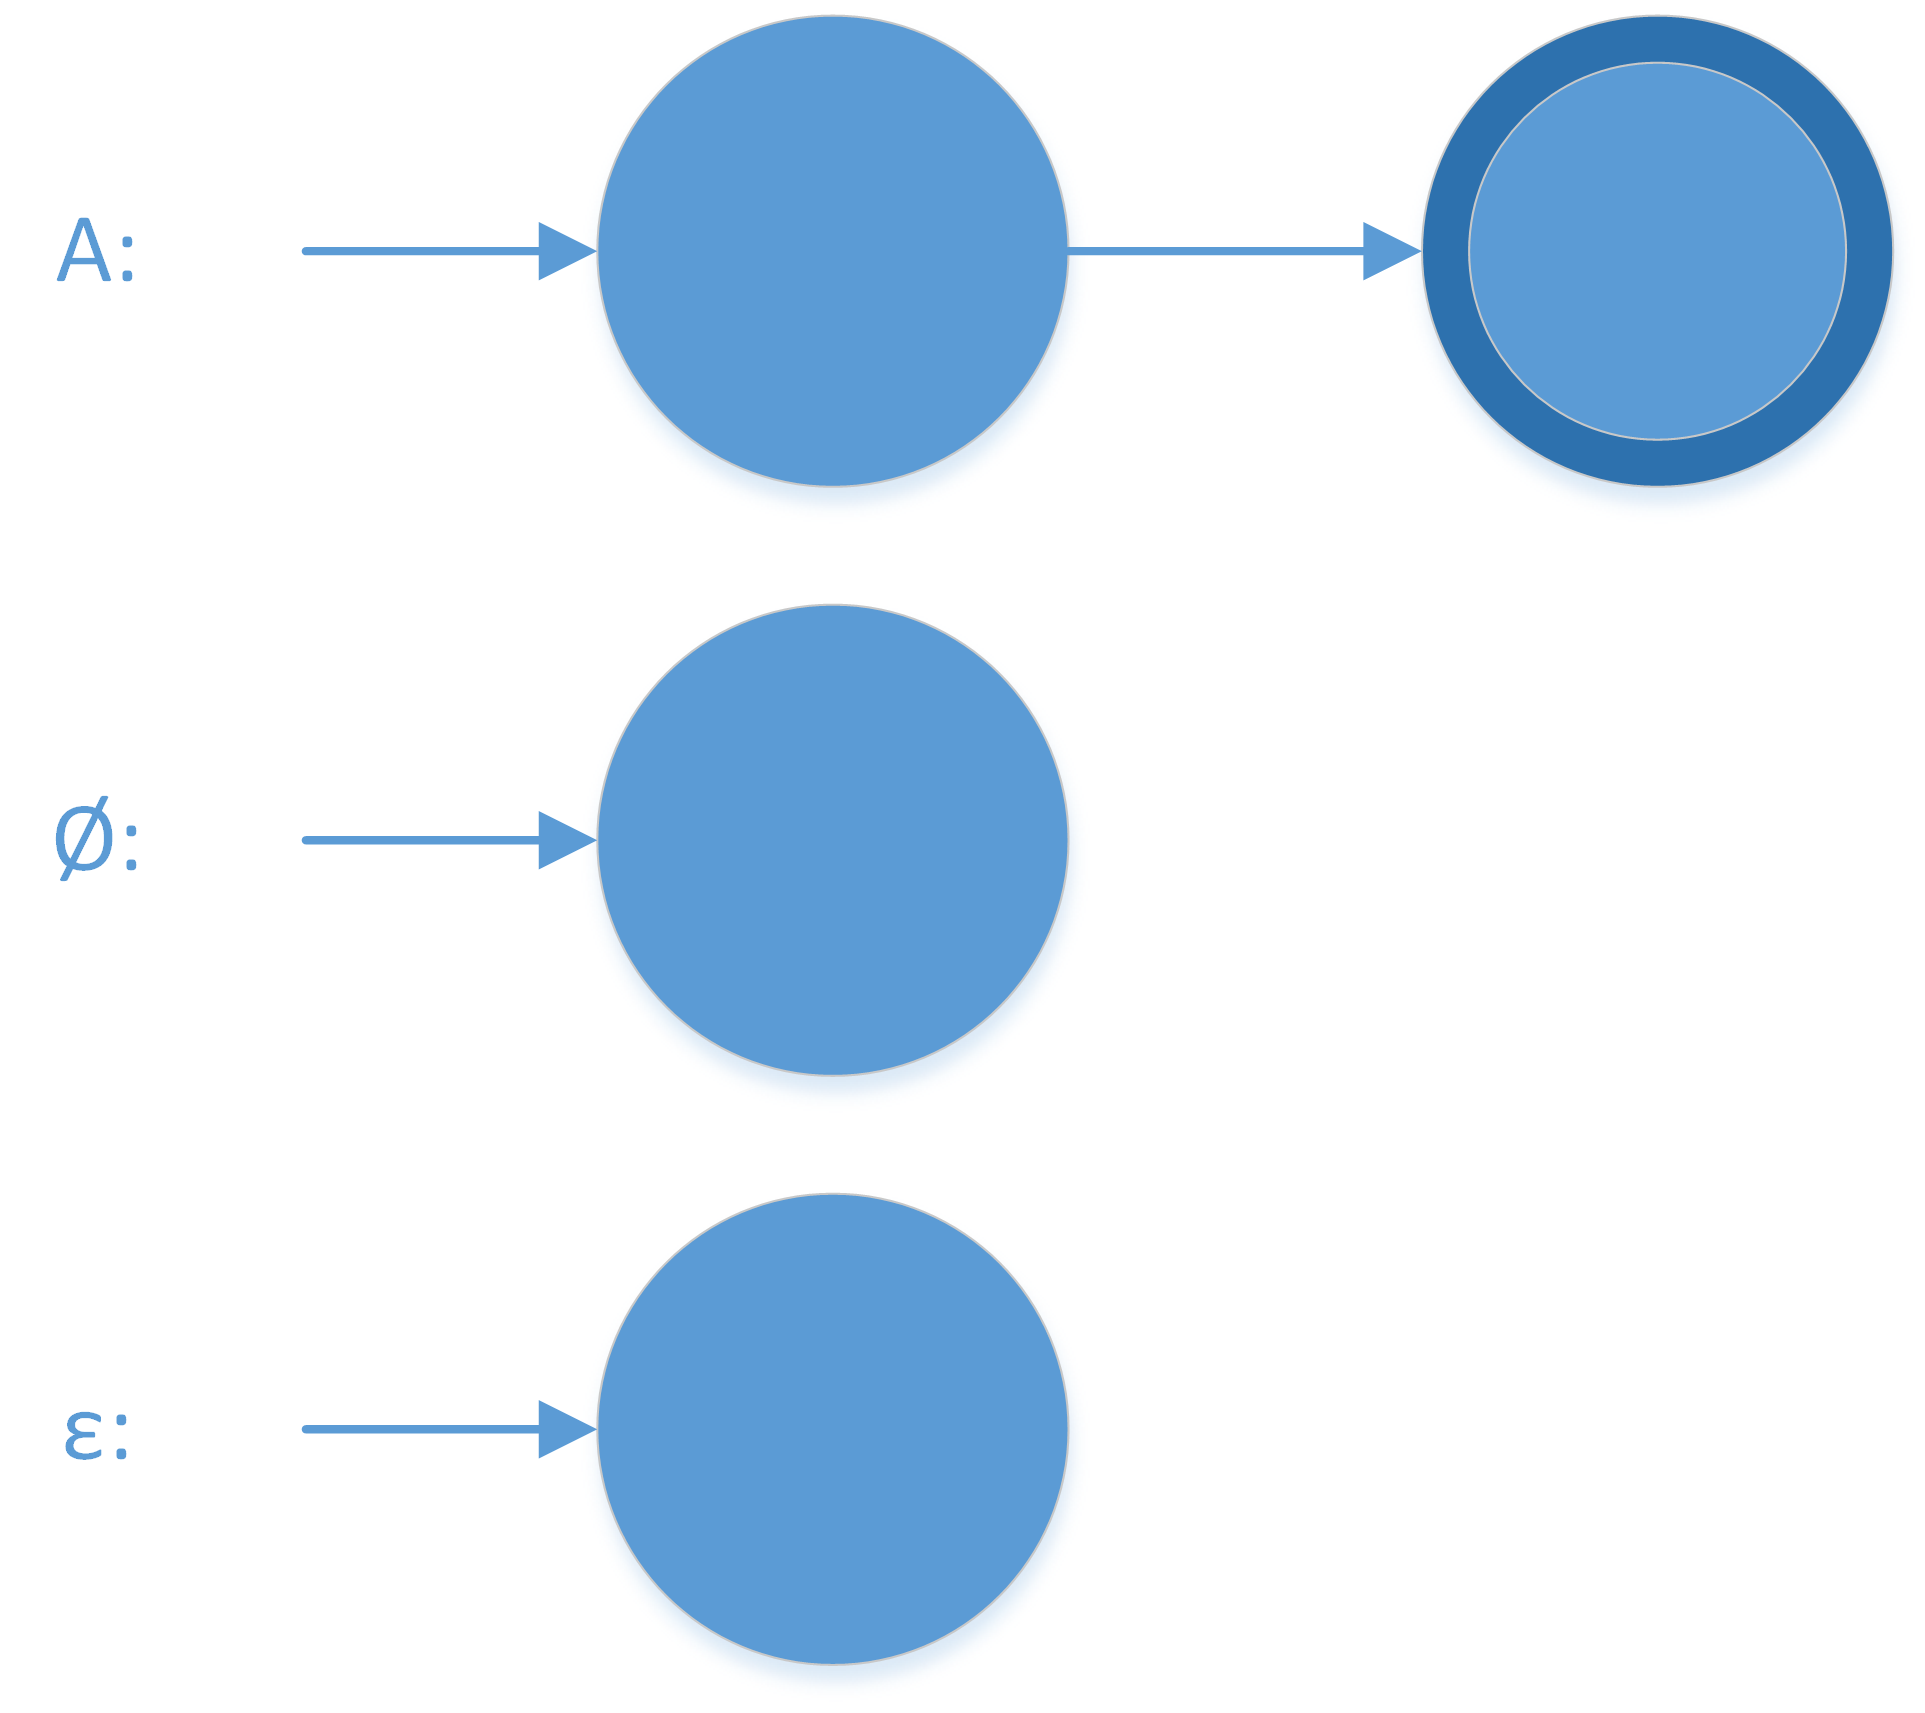
\includegraphics[width=60mm]{Fig1x.png}
}
\caption{Tre tilfælde ved basistrinnet}
\label{fig:fig1}
\end{figure}

\item[Skridt -- antag påstand for alle $k'<k$, vis for $k$:] 
Der er 3 tilfælde, som alle gør brug af at de regulære sprog er lukket
under de regulære operationer.

\begin{description}
\item[$R = (R_1 \cup R_2)$:] Da der findes per induktionsantagelse en
  $N_1, N_2$ så $L(R_1)=L(N_1)$, $L(R_2)=L(N_2)$. Vi skal lave en NFA
  der genkender $L(N_1) \cup L(N_2)$, og det er muligt da de regulære
  udtryk er lukket under $\cup$. 
\item[$R = (R_1 \circ R_2)$:] Igen findes pr. induktionsantagelse
  $N_1, N_2$ så $L(R_1) = L(N_1), L(R_2)=L(N_2)$, og det er muligt at
  konstruere en NFA $N$ så $L(N_1) \circ L(N_2)$.
  de regulære sprog er lukket under $\circ$.
\item[$(R)^*$:] Pr. induktionsantagelse findes en NFA $N$ så
  $L(R)=L(N)$. Vi kan lave en NFA som genkender $(L(N))^*$ da de
  regulære udtryk er lukket under $*$
\end{description}
\end{description}
\end{bevis}

\section{Eksempel}

Husk fra tidligere forelæsning konstruktionen af en NFA for $L^*$ (se
Figur \ref{fig:fig2}) samt $\circ$-konstruktionen (se Figur
\ref{fig:fig3}).

\begin{figure}[H]%skal placeres rigtigt
{\centering 
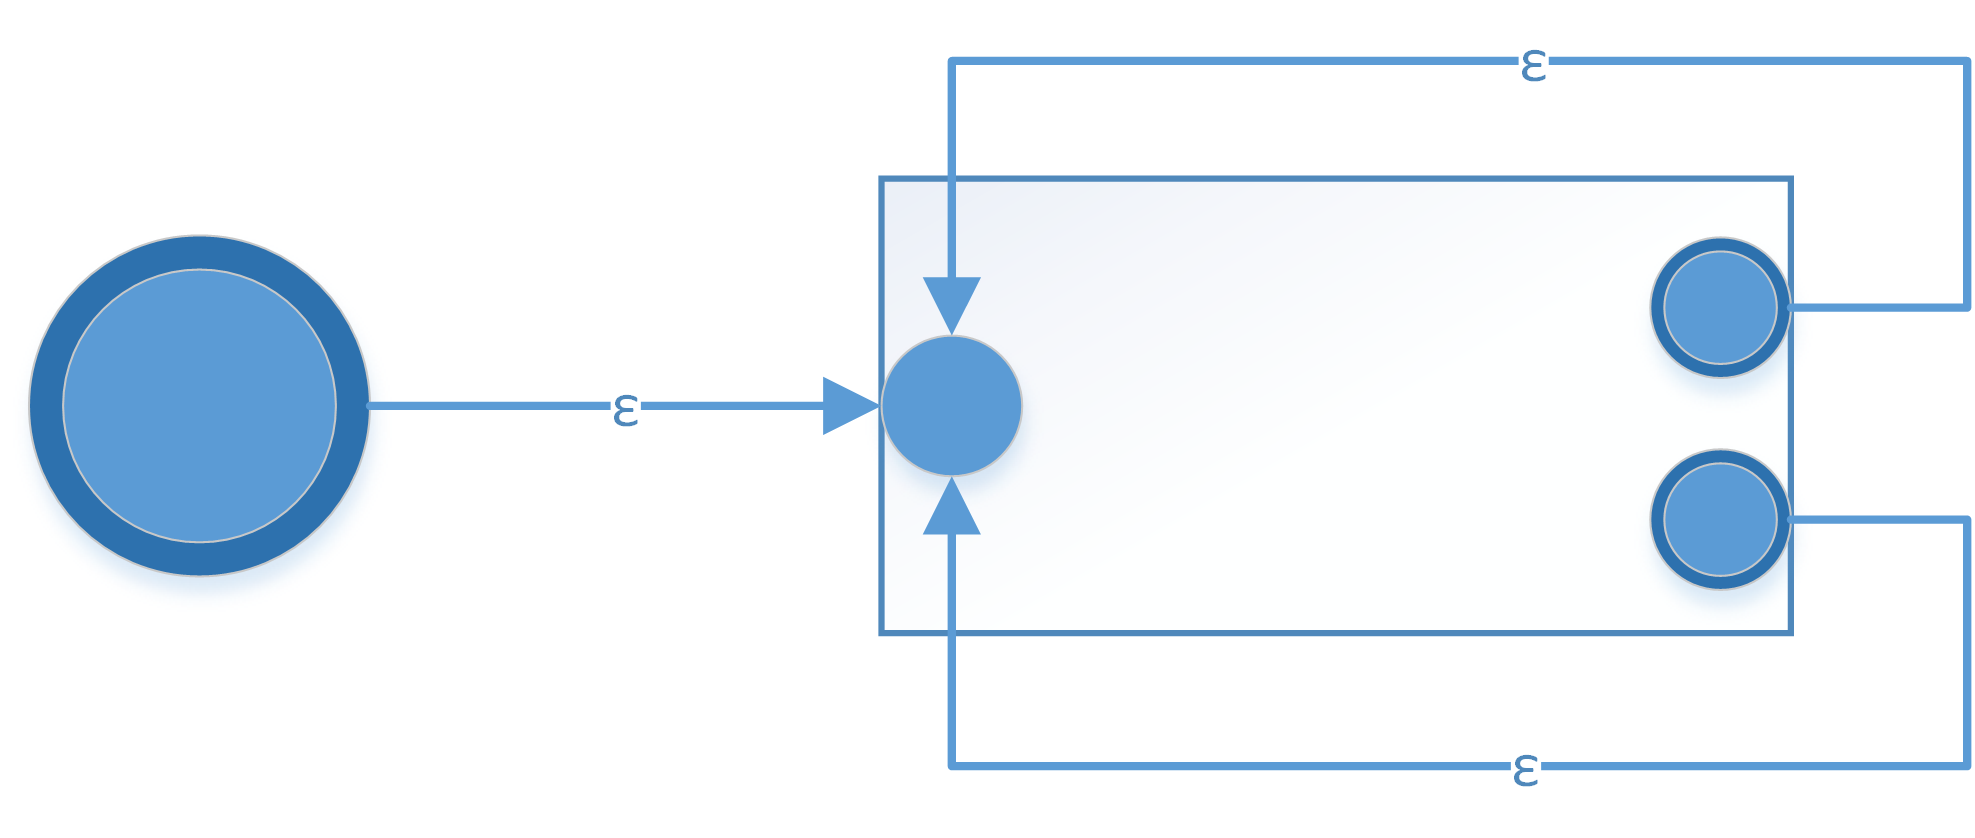
\includegraphics[width=100mm]{Fig2x.png}
}
\caption{*-konstruktion af NFA}
\label{fig:fig2}
\end{figure}

\begin{figure}[H]%skal placeres rigtigt
{\centering 
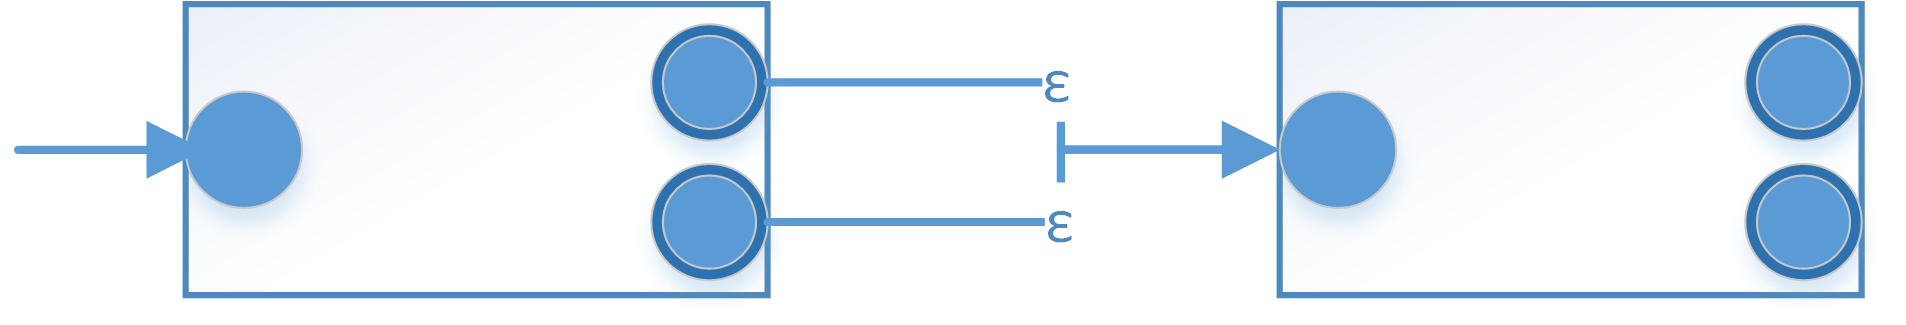
\includegraphics[width=\textwidth]{Fig3x.png}
}
\caption{$\circ$-konstruktionen af NFA}
\label{fig:fig3}
\end{figure}

\begin{eksempel}
Betragt det regulære udtryk $\mathbf{1^*0(1^*01^*01^*)^*  \cup (1 \cup 0)^*11}$

For at konstruere en NFA fra dette regulære udtryk starter man med at
konstruere NFA'er for de mindste bestanddele, og anvender derefter
konstruktionerne for de regulære operationer. I dette tilfælde starter
man altså med at konstruere en NFA for $\mathbf{0}$ og $\mathbf{1}$, som set på Figur
\ref{fig:fig4}.

\begin{figure}[H]%skal placeres rigtigt
{\centering 
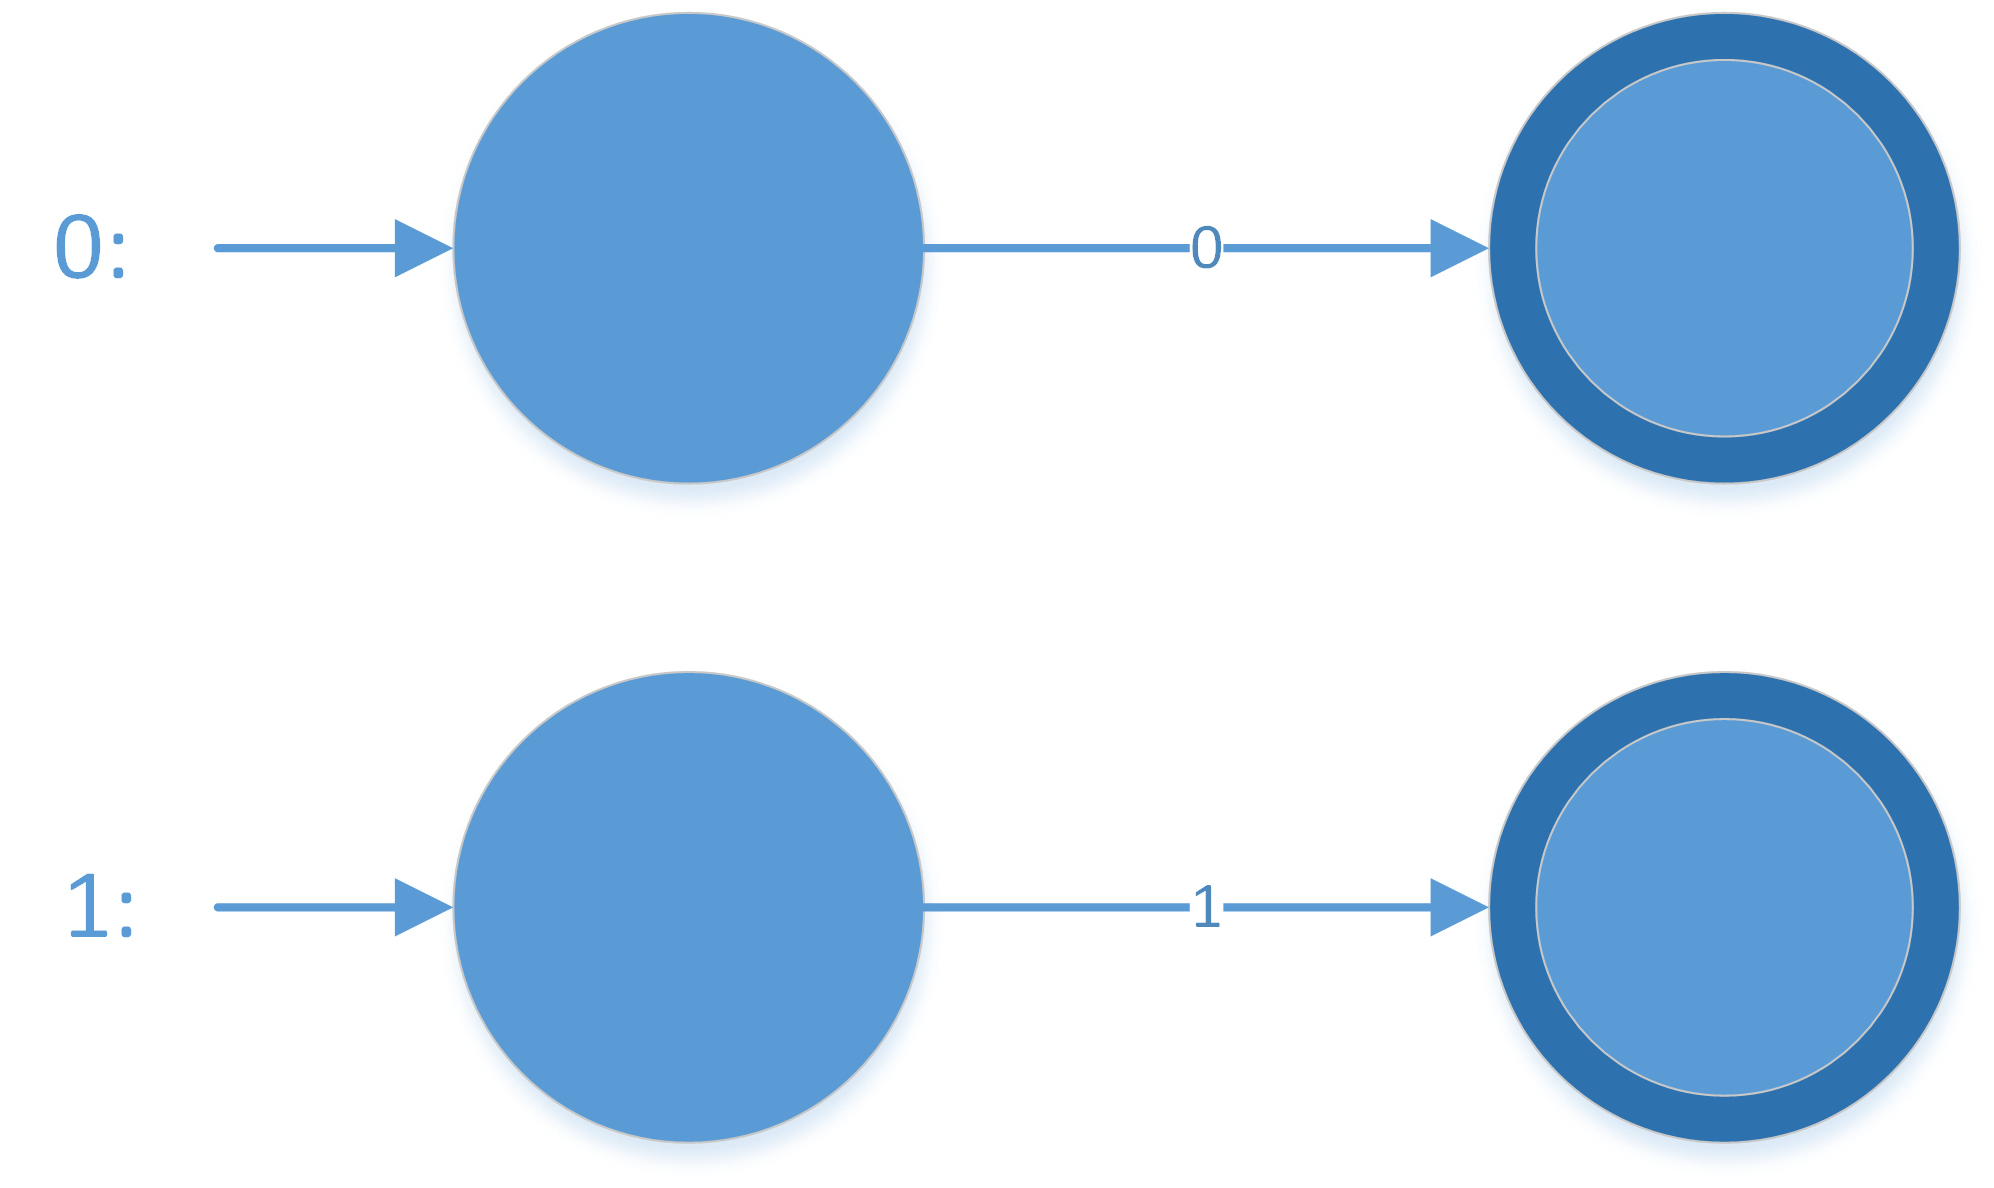
\includegraphics[width=\textwidth]{Fig4x.png}
}
\caption{NFA'er for $\mathbf{0}$ og $\mathbf{1}$}
\label{fig:fig4}
\end{figure}

Herefter konstrueres NFA'en for $\mathbf{1^*}$ som set på Figur \ref{fig:fig5}. 

\begin{figure}[H]%skal placeres rigtigt
{\centering 
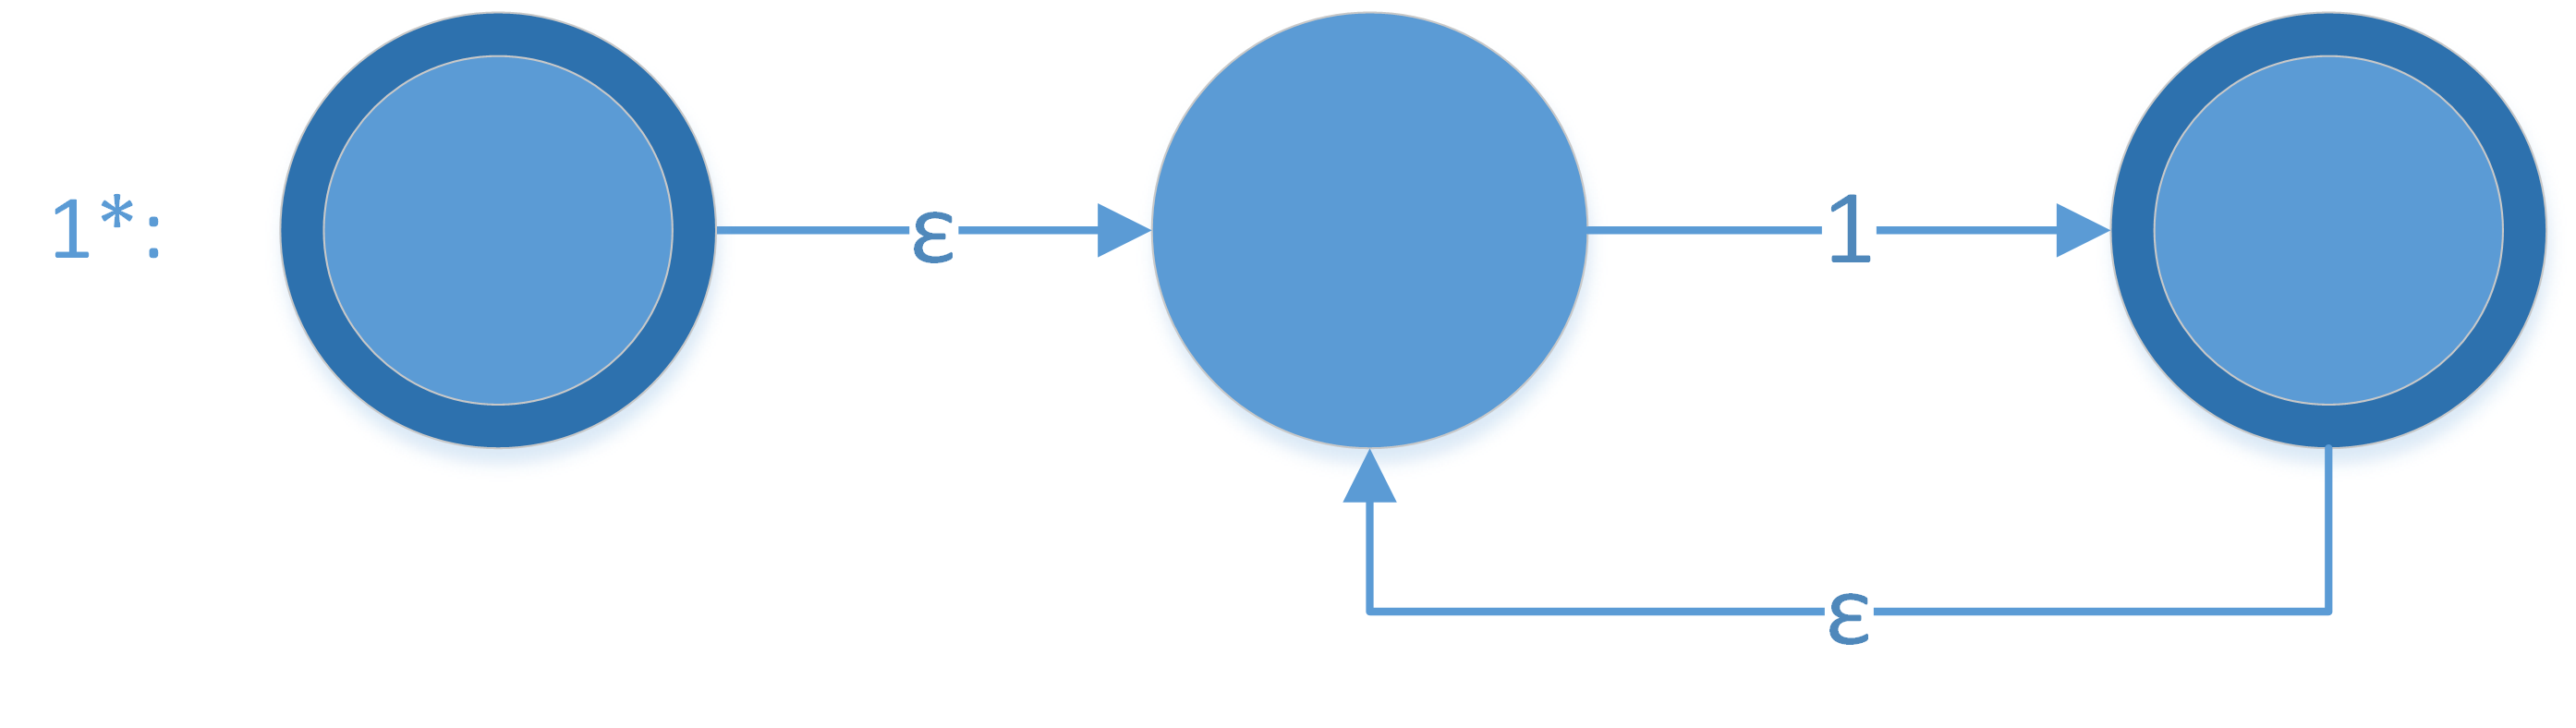
\includegraphics[width=\textwidth]{Fig5x.png}
} \caption{NFA for $\mathbf{1^*}$}
\label{fig:fig5}
\end{figure}

Herefter konstrueres NFA'en for $\mathbf{1^*0}$ som set på Figur \ref{fig:fig6}. 

\begin{figure}[H]%skal placeres rigtigt
{\centering 
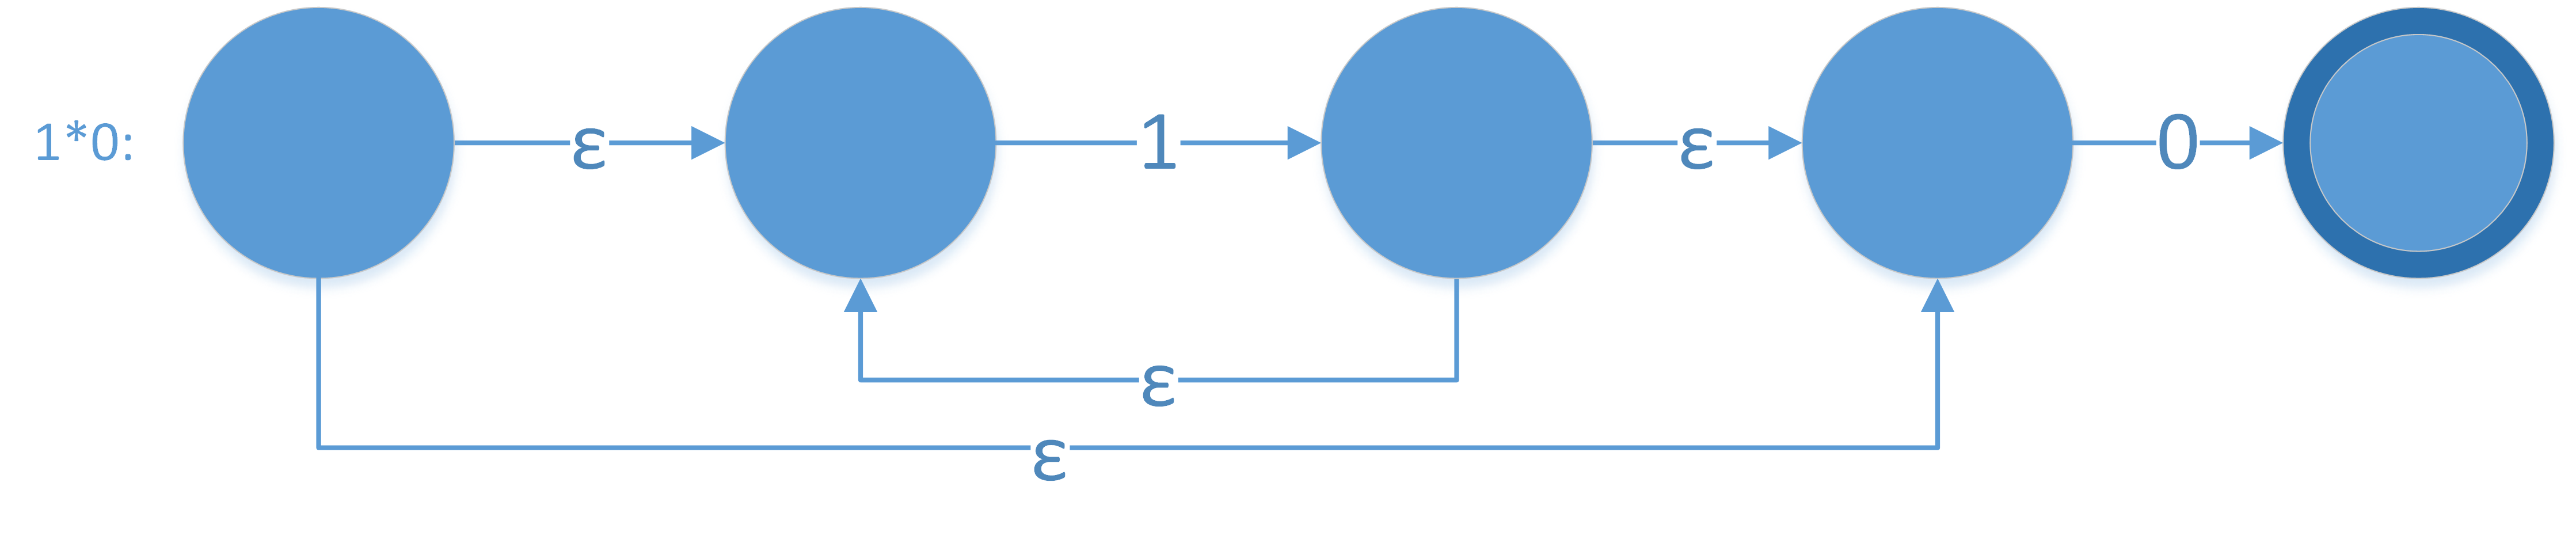
\includegraphics[width=\textwidth]{Fig6x.png}
} \caption{NFA for $\mathbf{1^*0}$}
\label{fig:fig6}
\end{figure}

Herefter konstrueres NFA'en for $\mathbf{1^*01^*0}$ som set på Figur \ref{fig:fig7}. 

\begin{figure}[H]%skal placeres rigtigt
{\centering 
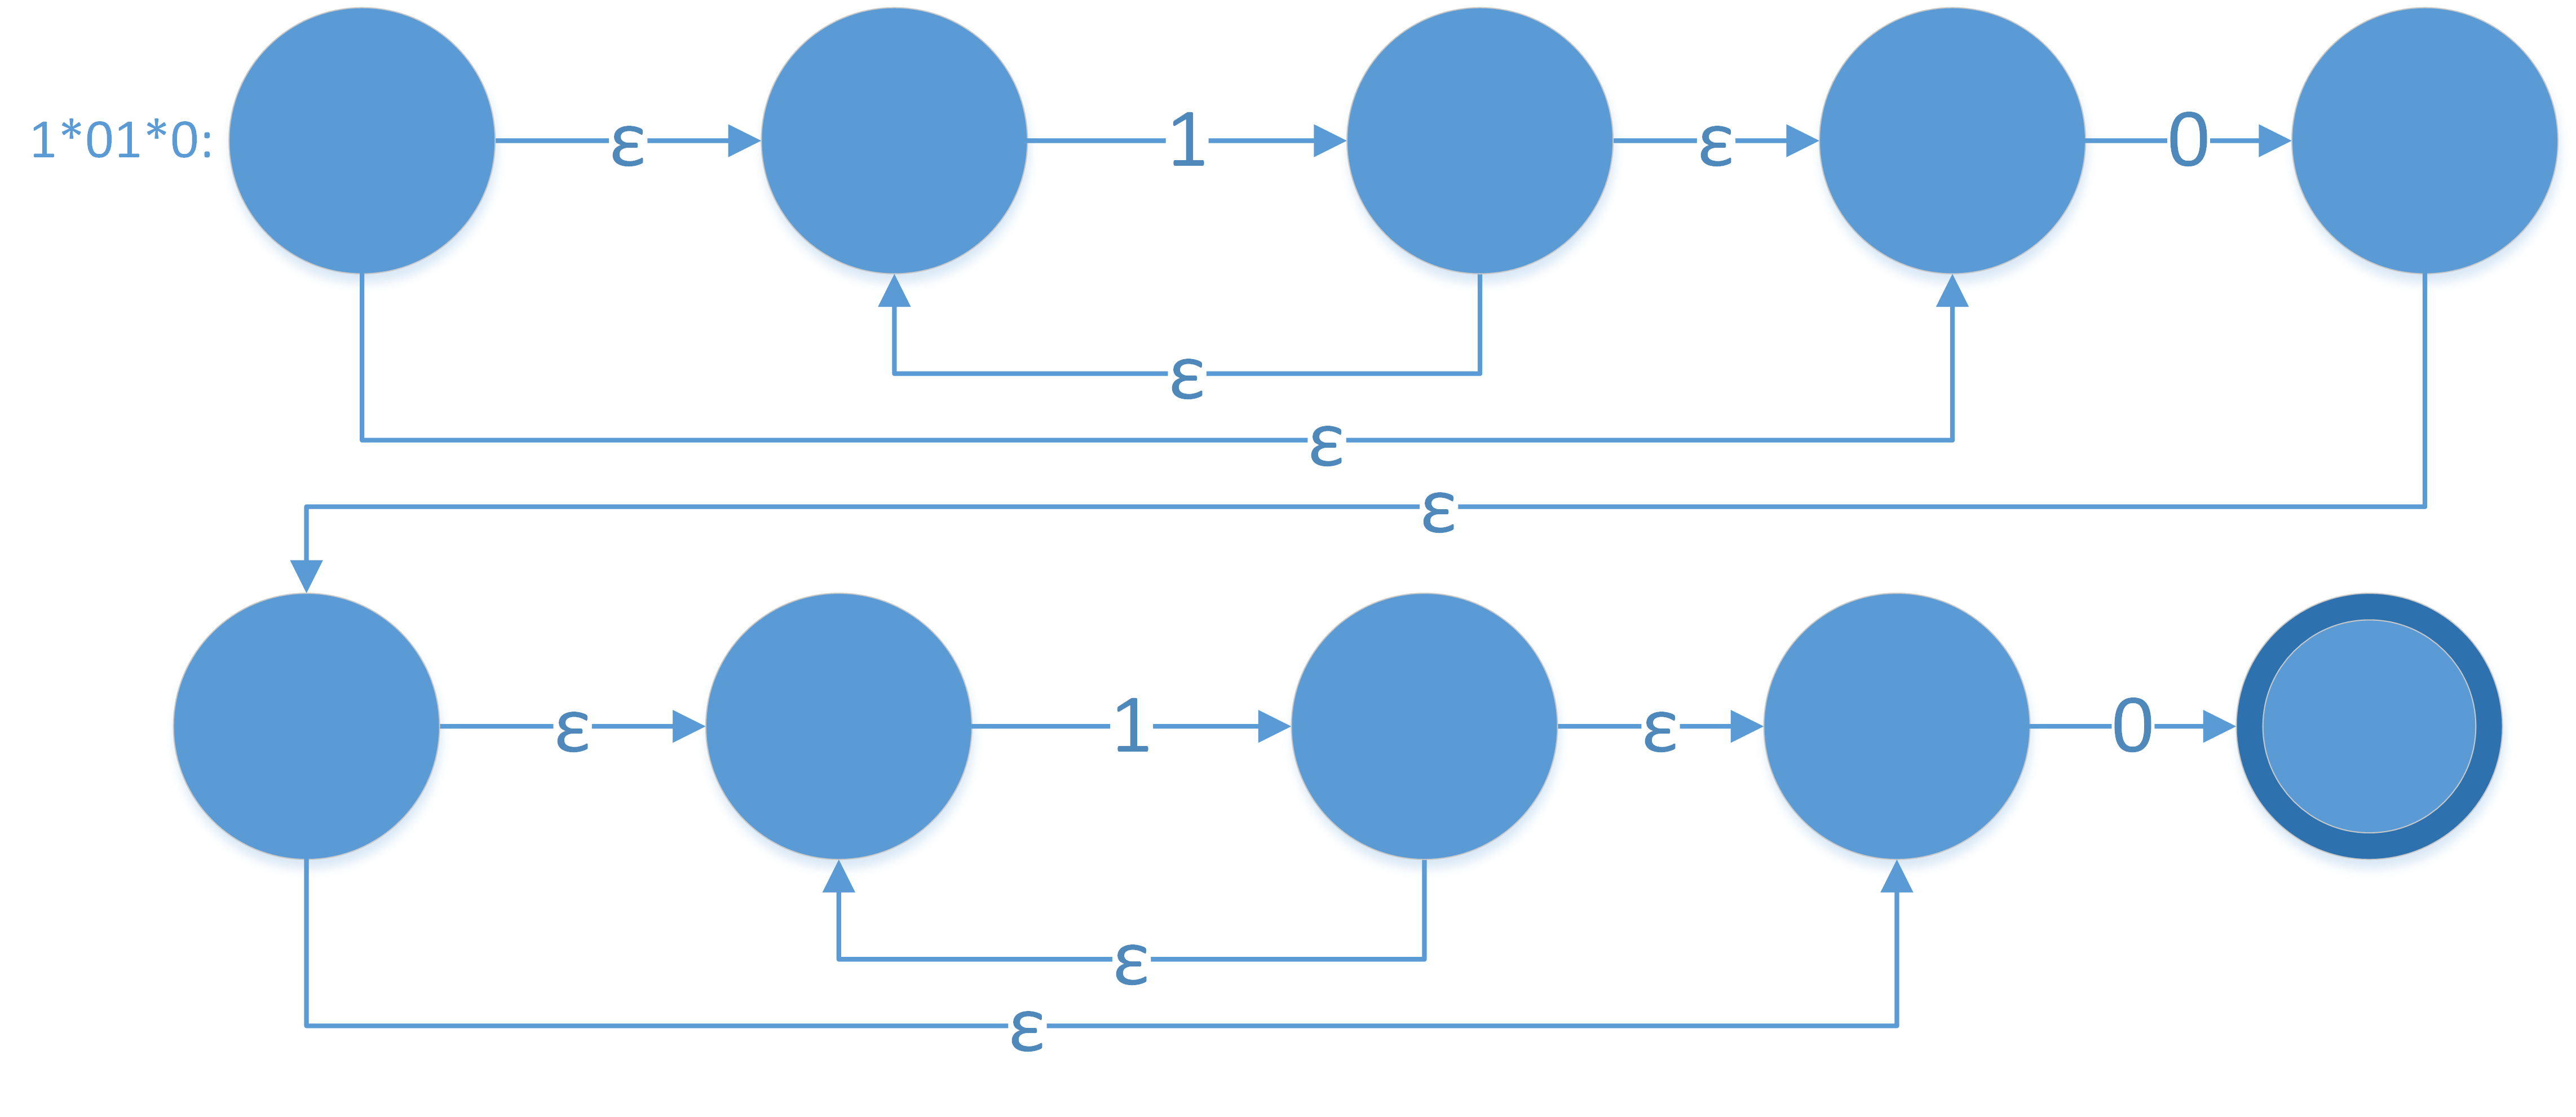
\includegraphics[width=\textwidth]{Fig7x.png}
} \caption{NFA for $\mathbf{1^*01^*0}$}
\label{fig:fig7}
\end{figure}

Herefter konstrueres NFA'en for $\mathbf{1^*01^*01^*}$ som set på Figur \ref{fig:fig8}. 

\begin{figure}[H]%skal placeres rigtigt
{\centering 
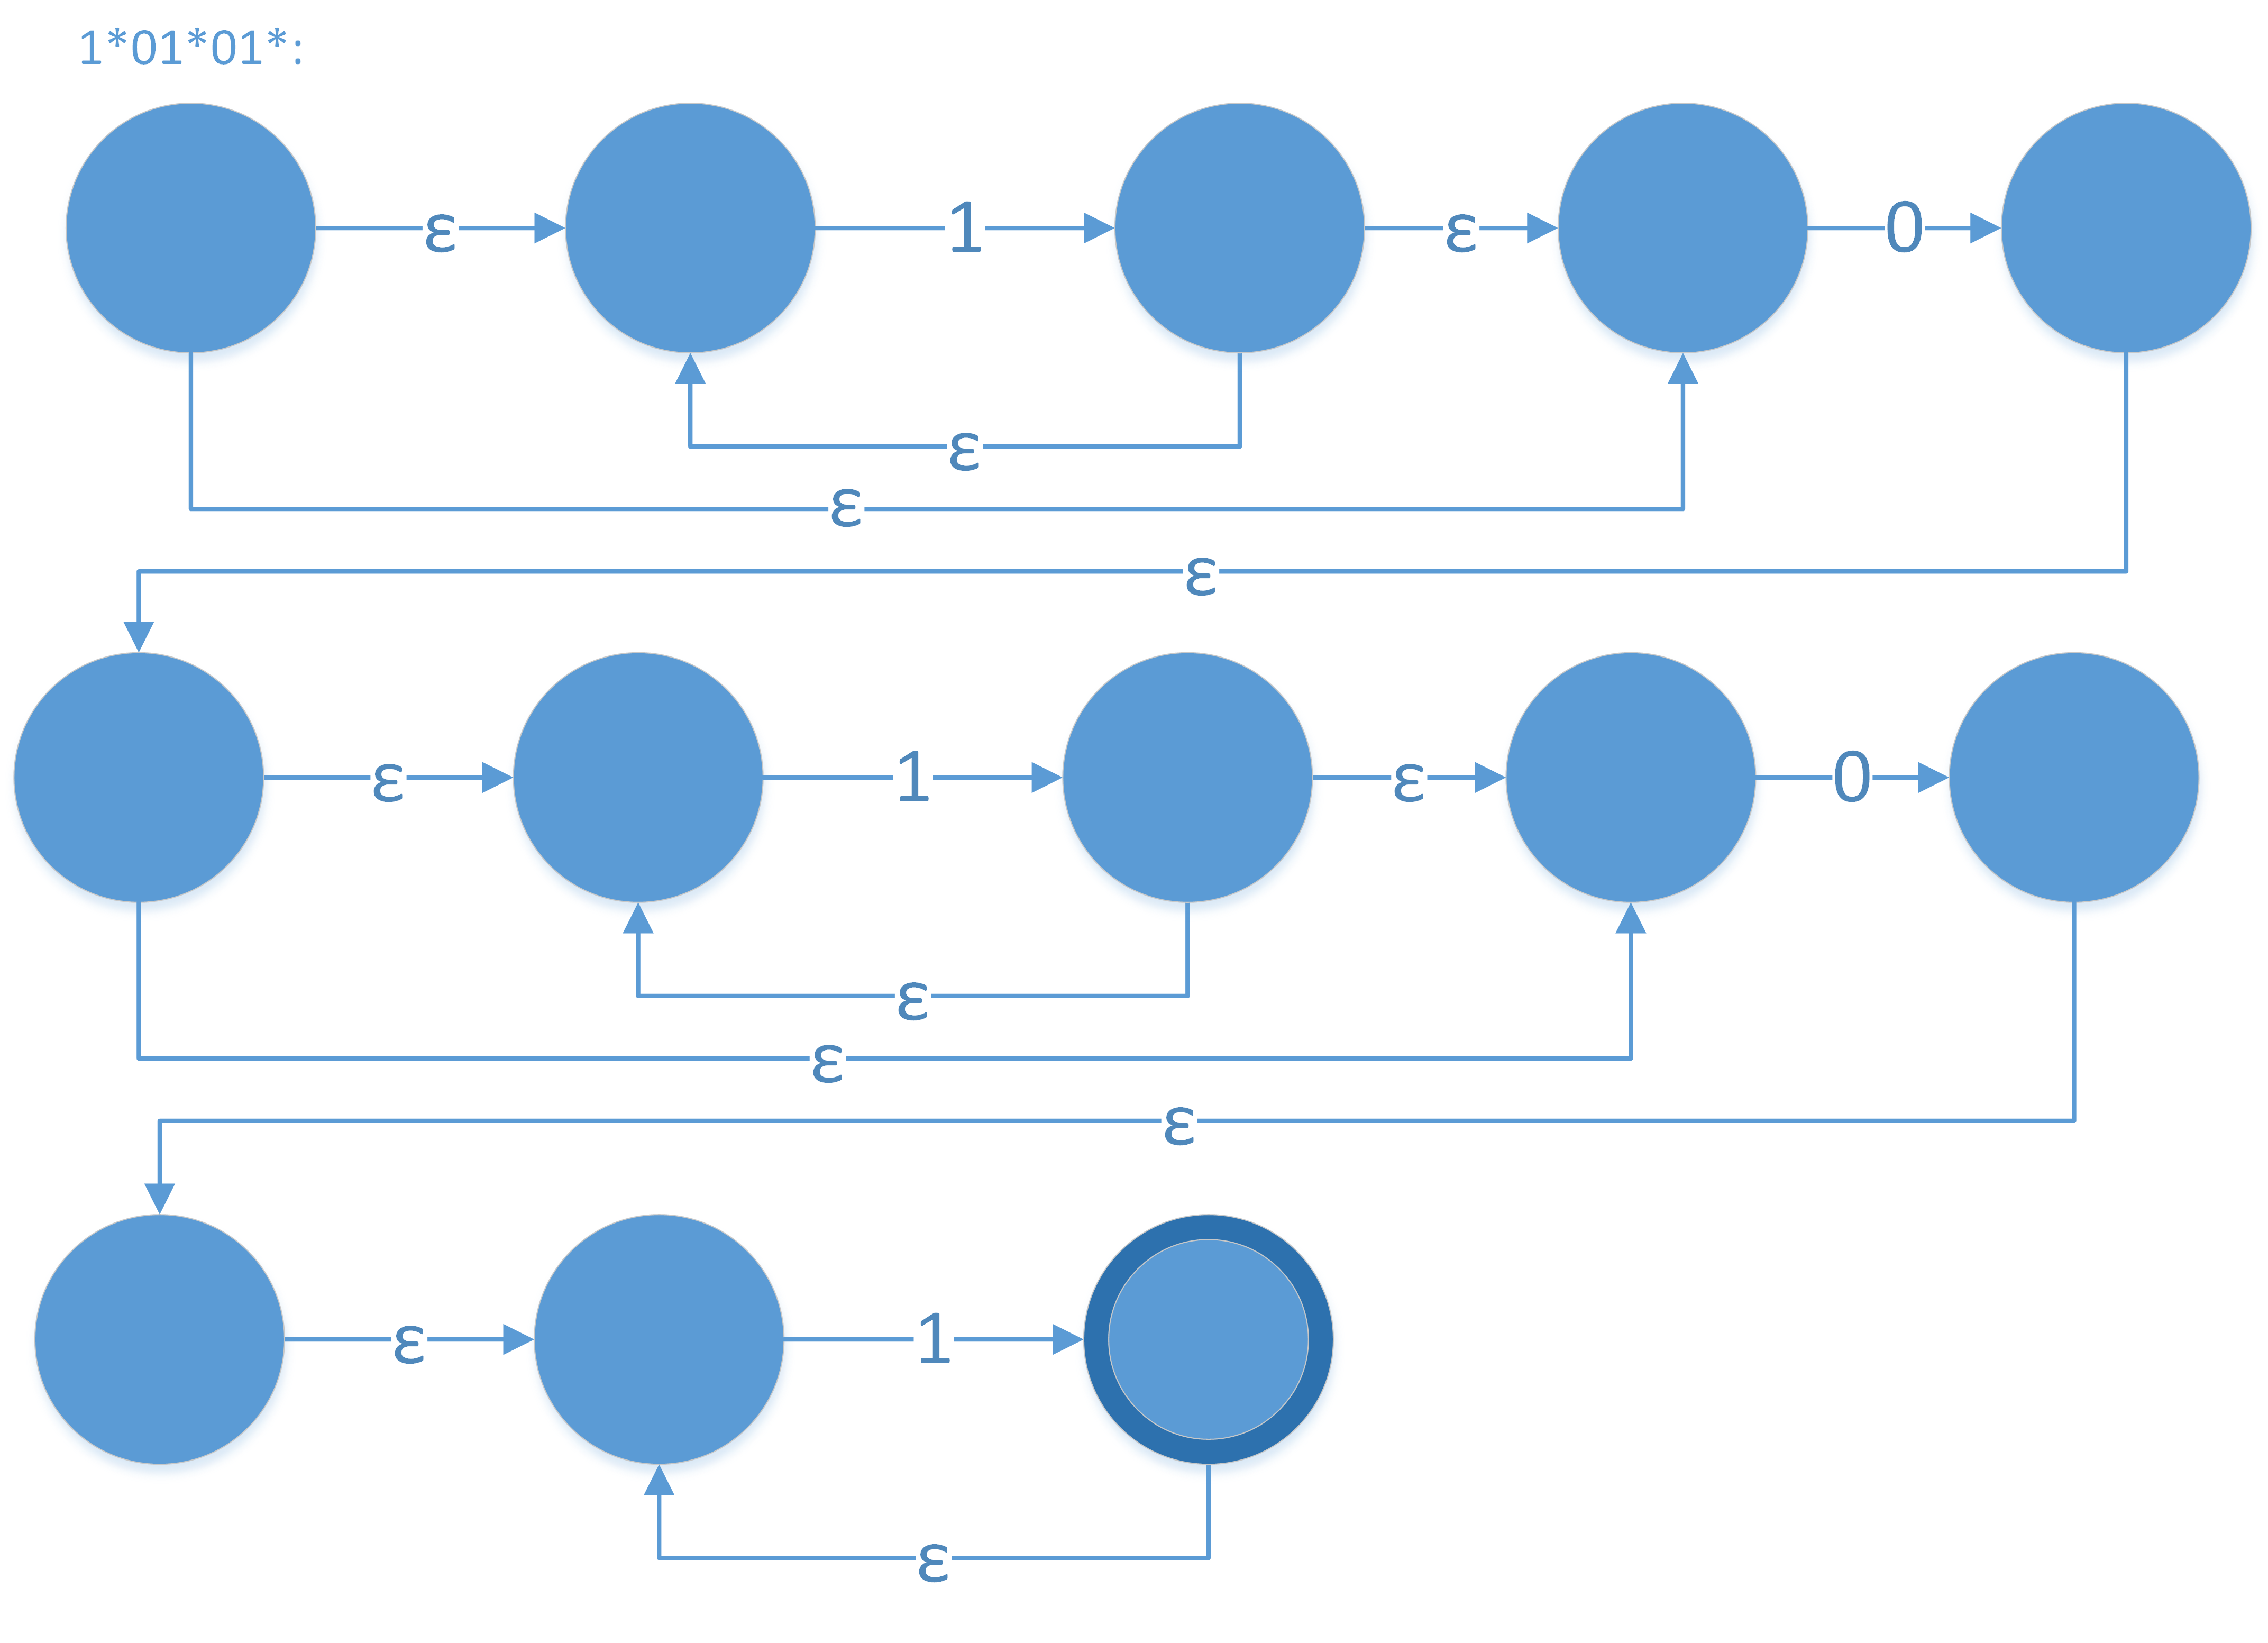
\includegraphics[width=\textwidth]{Fig8x.png}
} \caption{NFA for $\mathbf{1^*01^*01^*}$}
\label{fig:fig8}
\end{figure}

Herefter konstrueres NFA'en for $\mathbf{(1^*01^*01^*)^*}$ som set på Figur \ref{fig:fig9}. Denne NFA kaldes fremover $N$.

\begin{figure}[H]%skal placeres rigtigt
{\centering 
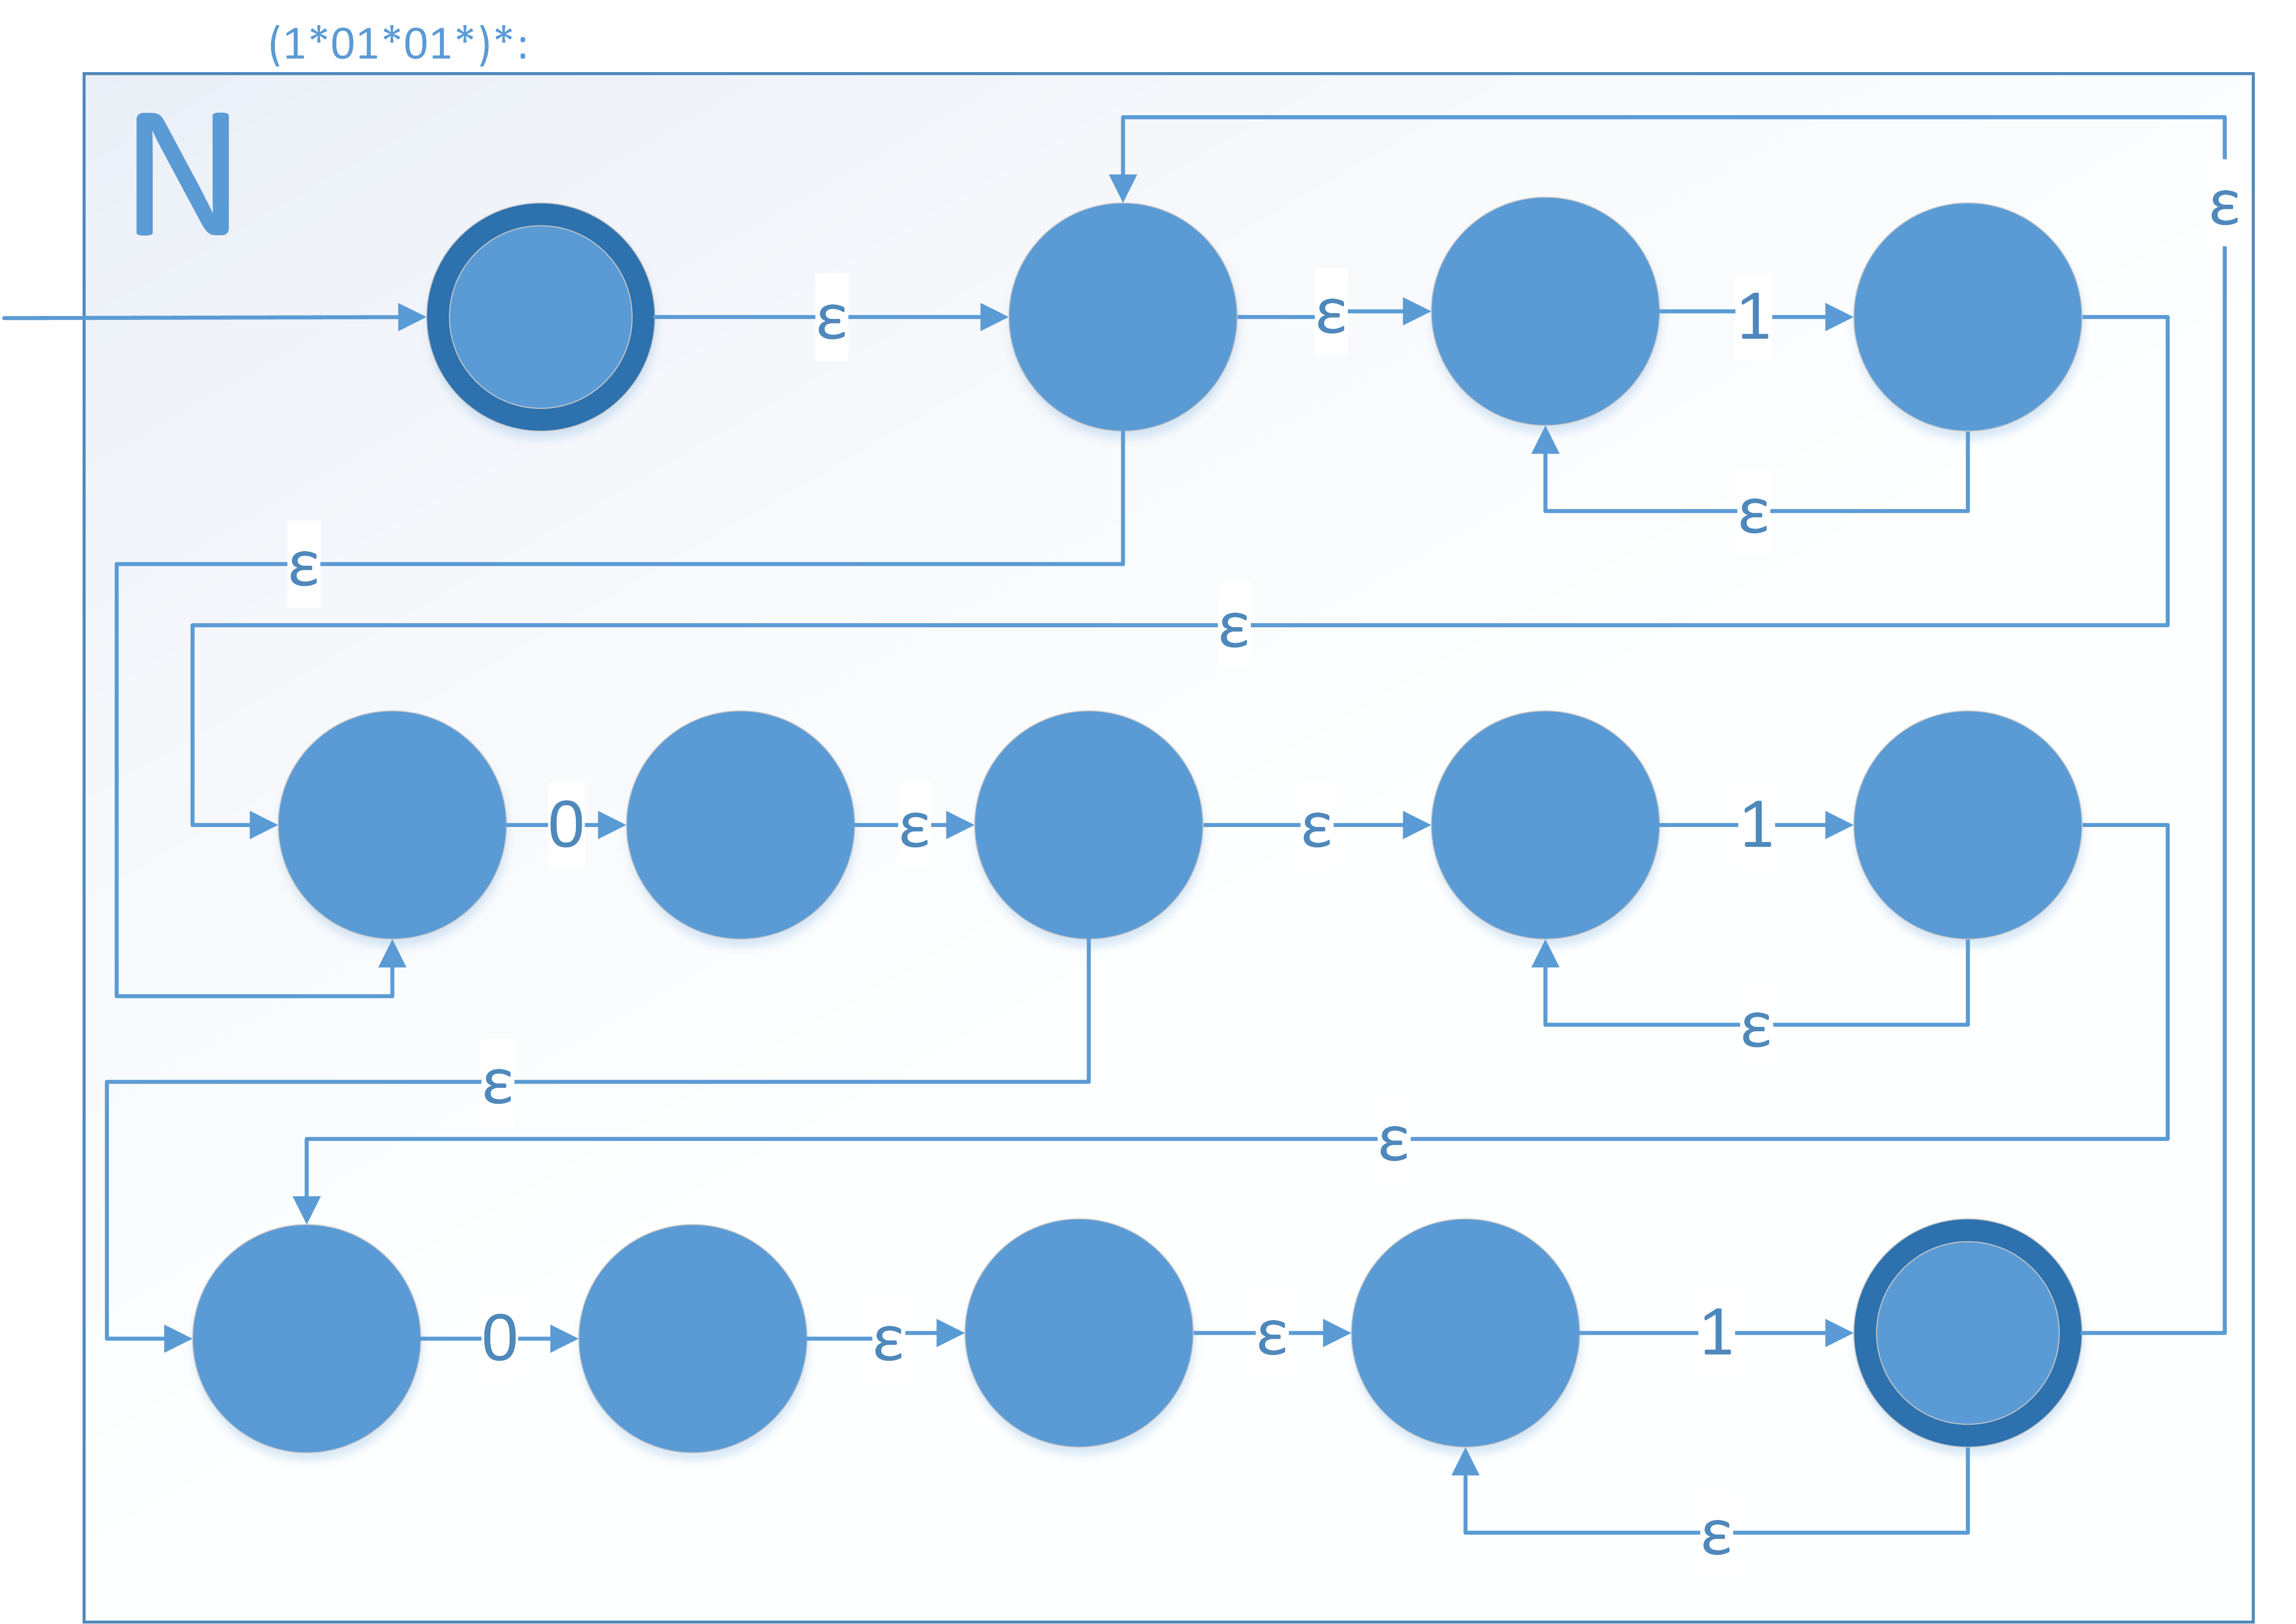
\includegraphics[width=\textwidth]{Fig9x.png}
} \caption{NFA for $\mathbf{(1^*01^*01^*)^*}$}
\label{fig:fig9}
\end{figure}

Herefter konstrueres NFA'en for $\mathbf{1*0(1^*01^*01^*)^*}$ som set på Figur \ref{fig:fig10}. Denne NFA kaldes fremover $N'$.

\begin{figure}[H]%skal placeres rigtigt
{\centering 
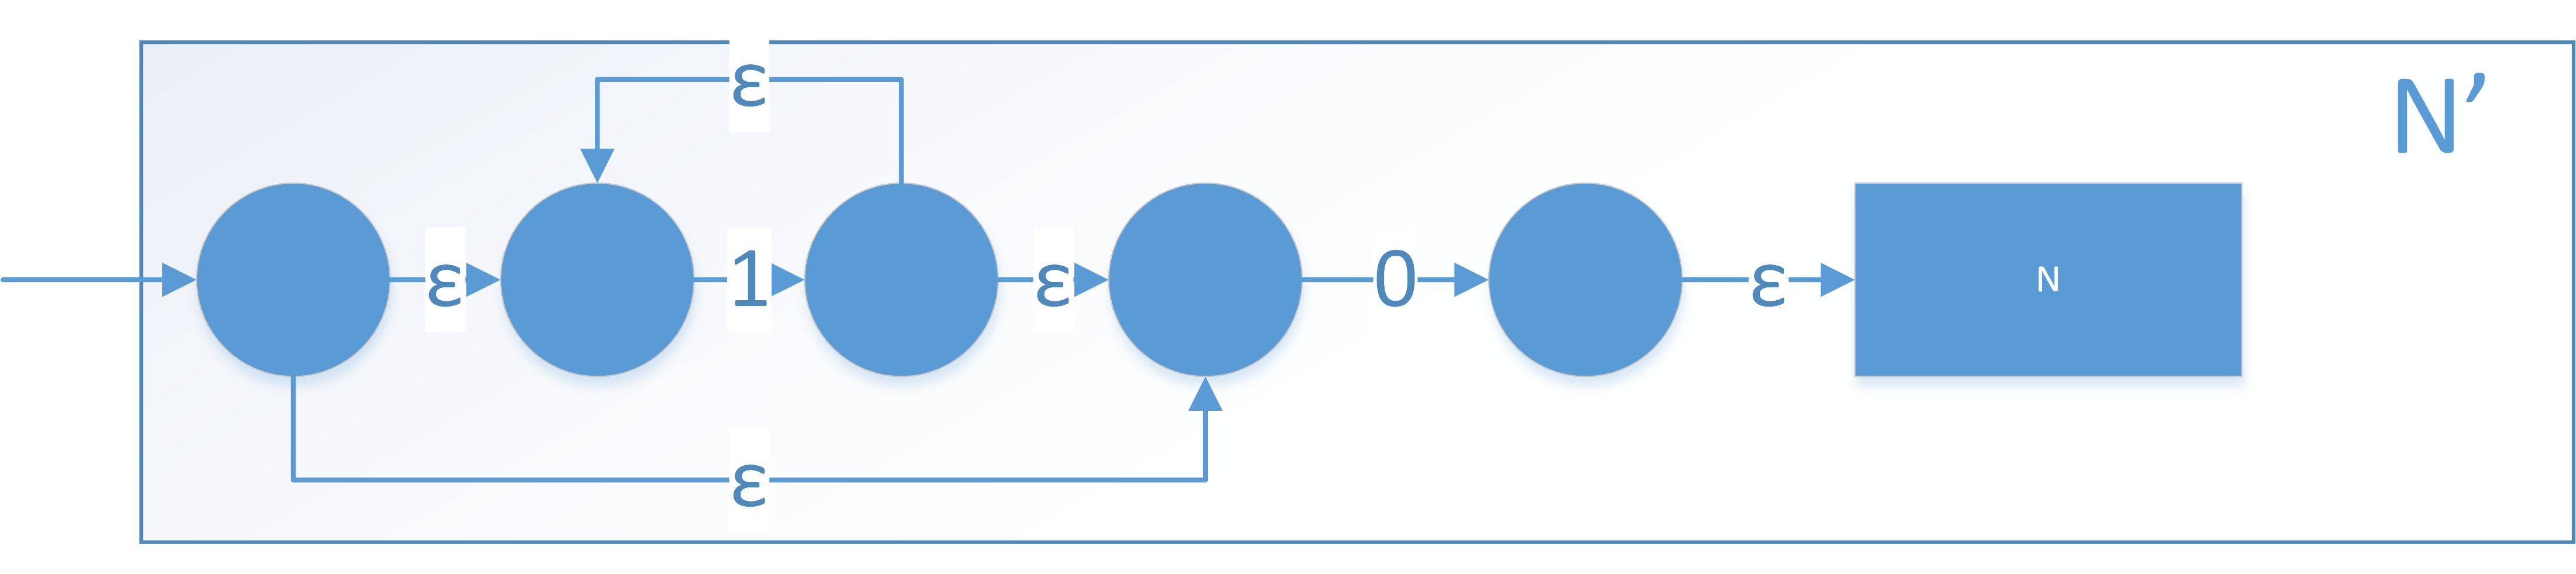
\includegraphics[width=\textwidth]{Fig10x.png}
} \caption{NFA for $\mathbf{1^*0(1^*01^*01^*)^*}$}
\label{fig:fig10}
\end{figure}

Herefter konstrueres NFA'en for $\mathbf{0\cup 1}$ som set på Figur \ref{fig:fig11}.

\begin{figure}[H]%skal placeres rigtigt
{\centering 
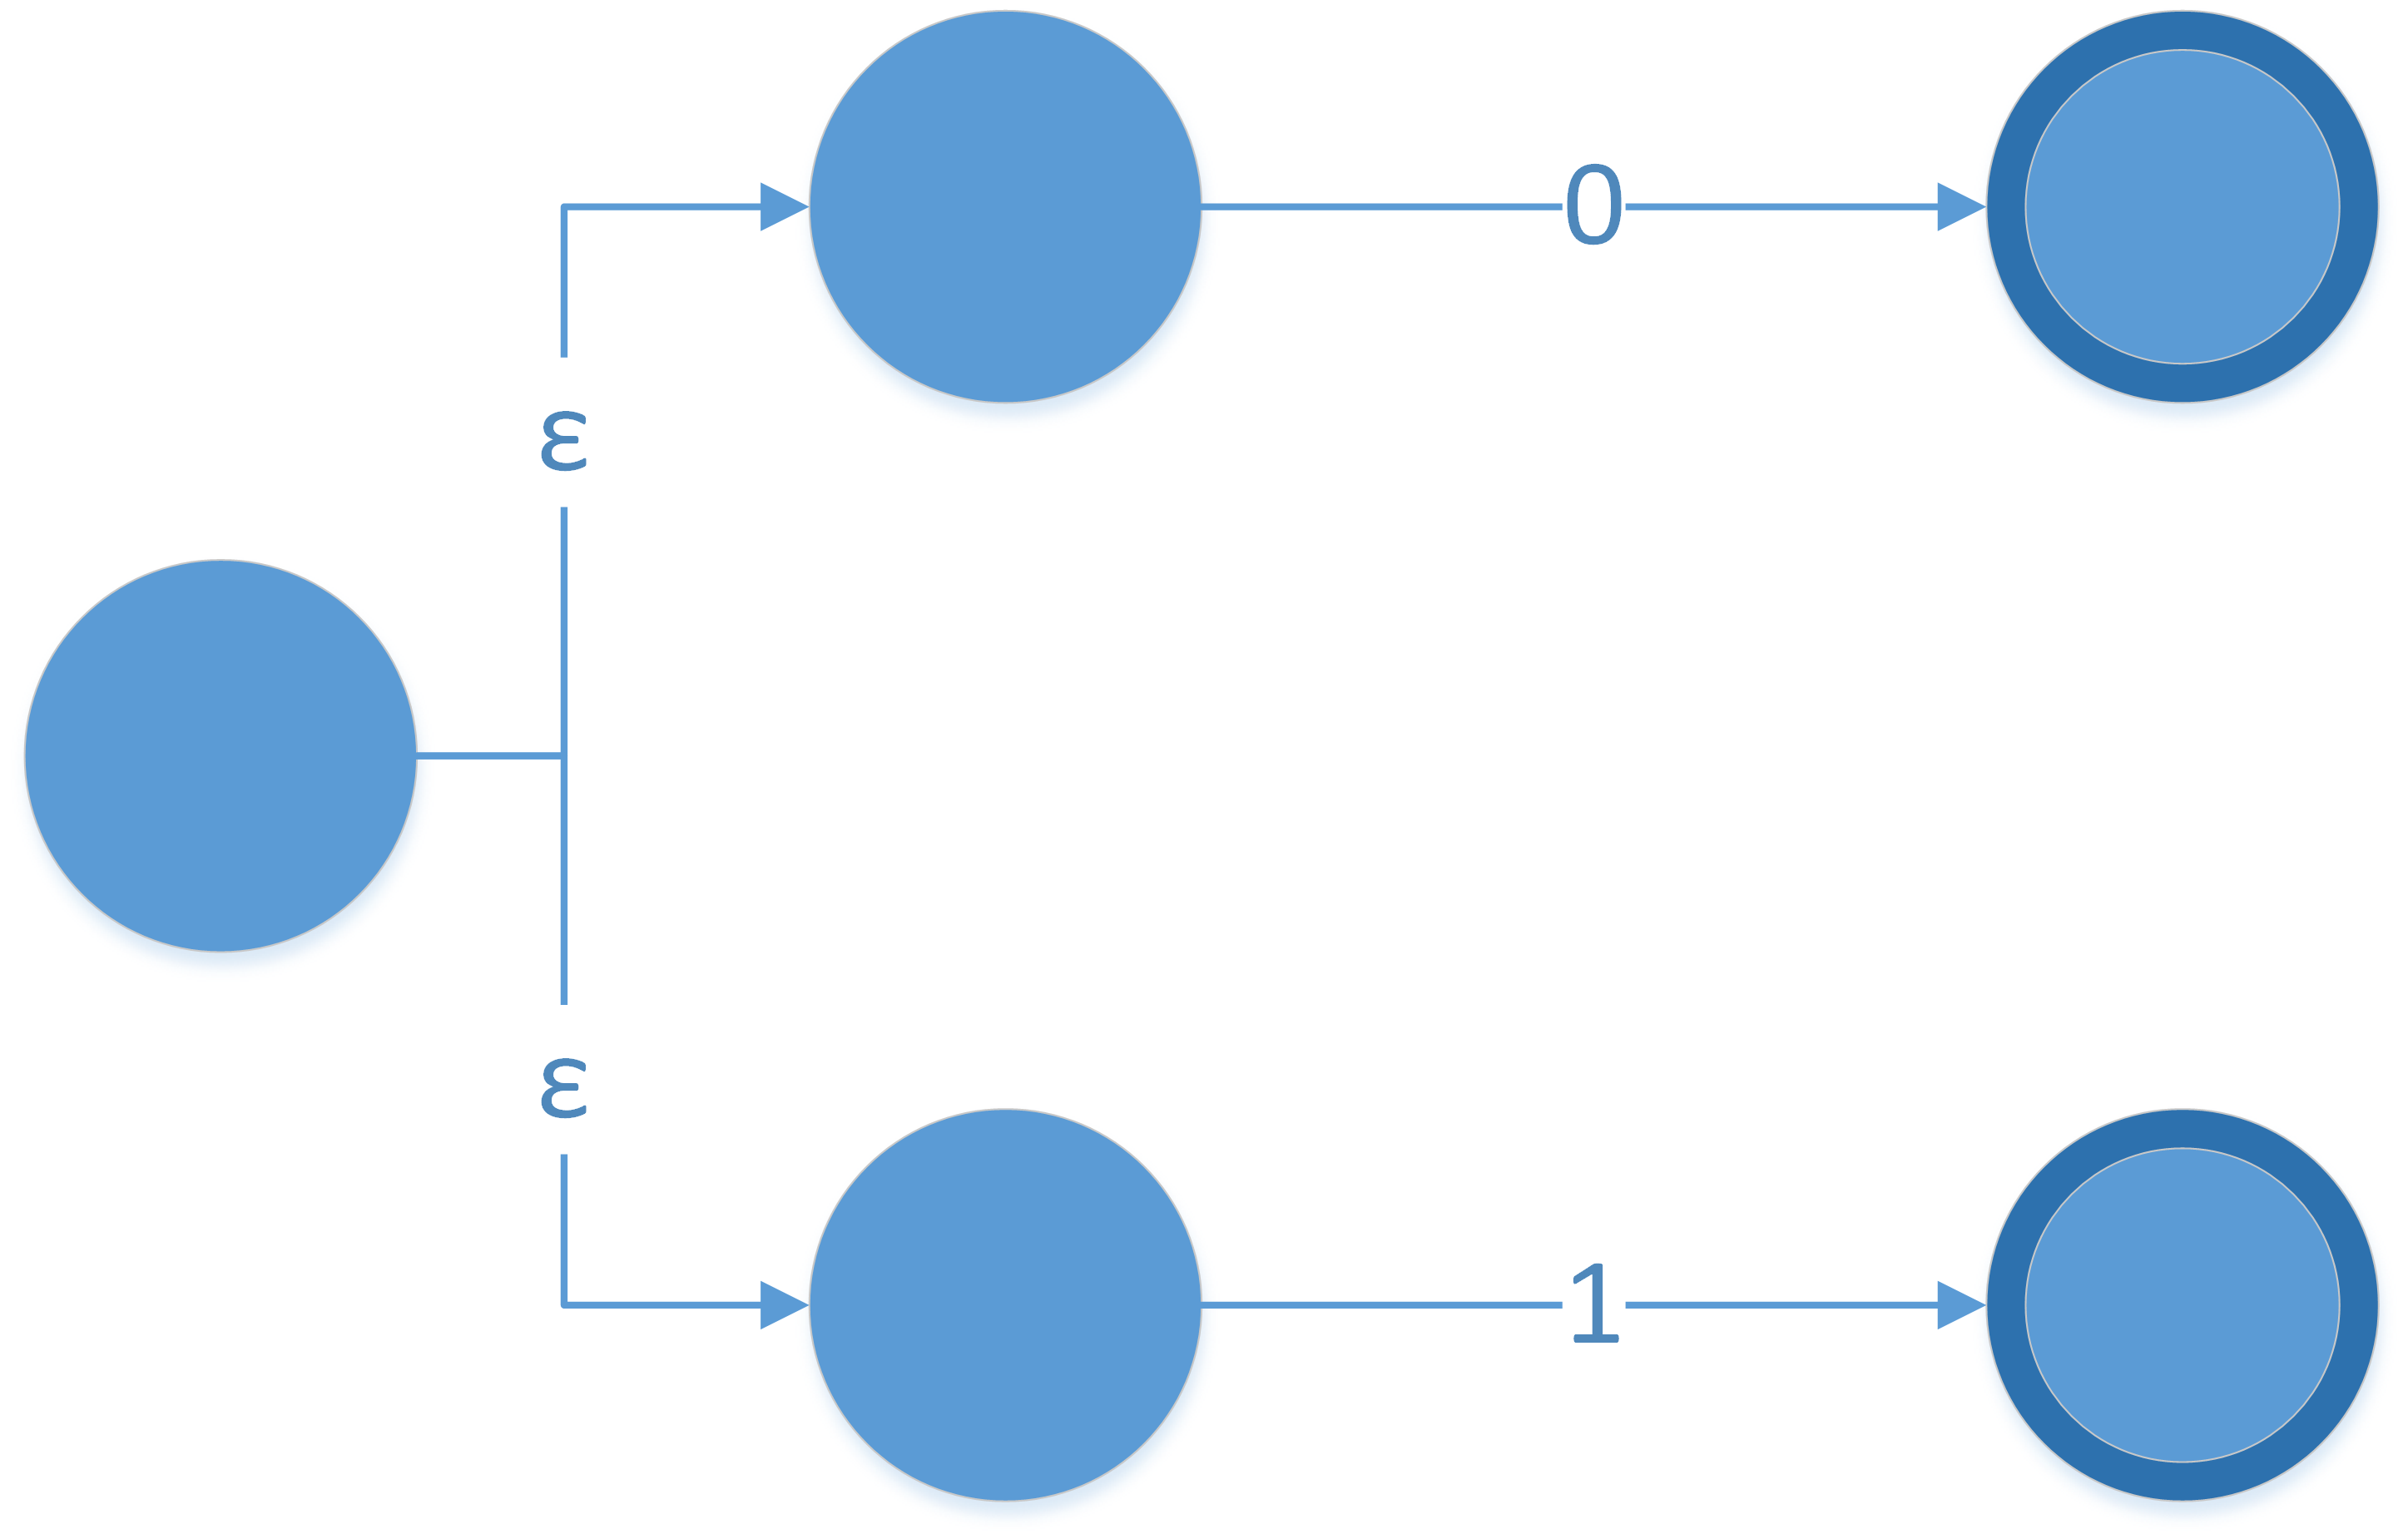
\includegraphics[width=\textwidth]{Fig11x.png}
} \caption{NFA for $\mathbf{0\cup 1}$}
\label{fig:fig11}
\end{figure}
Herefter konstrueres NFA'en for $\mathbf{(0\cup 1)^*}$ som set på Figur \ref{fig:fig12}.

\begin{figure}[H]%skal placeres rigtigt
{\centering 
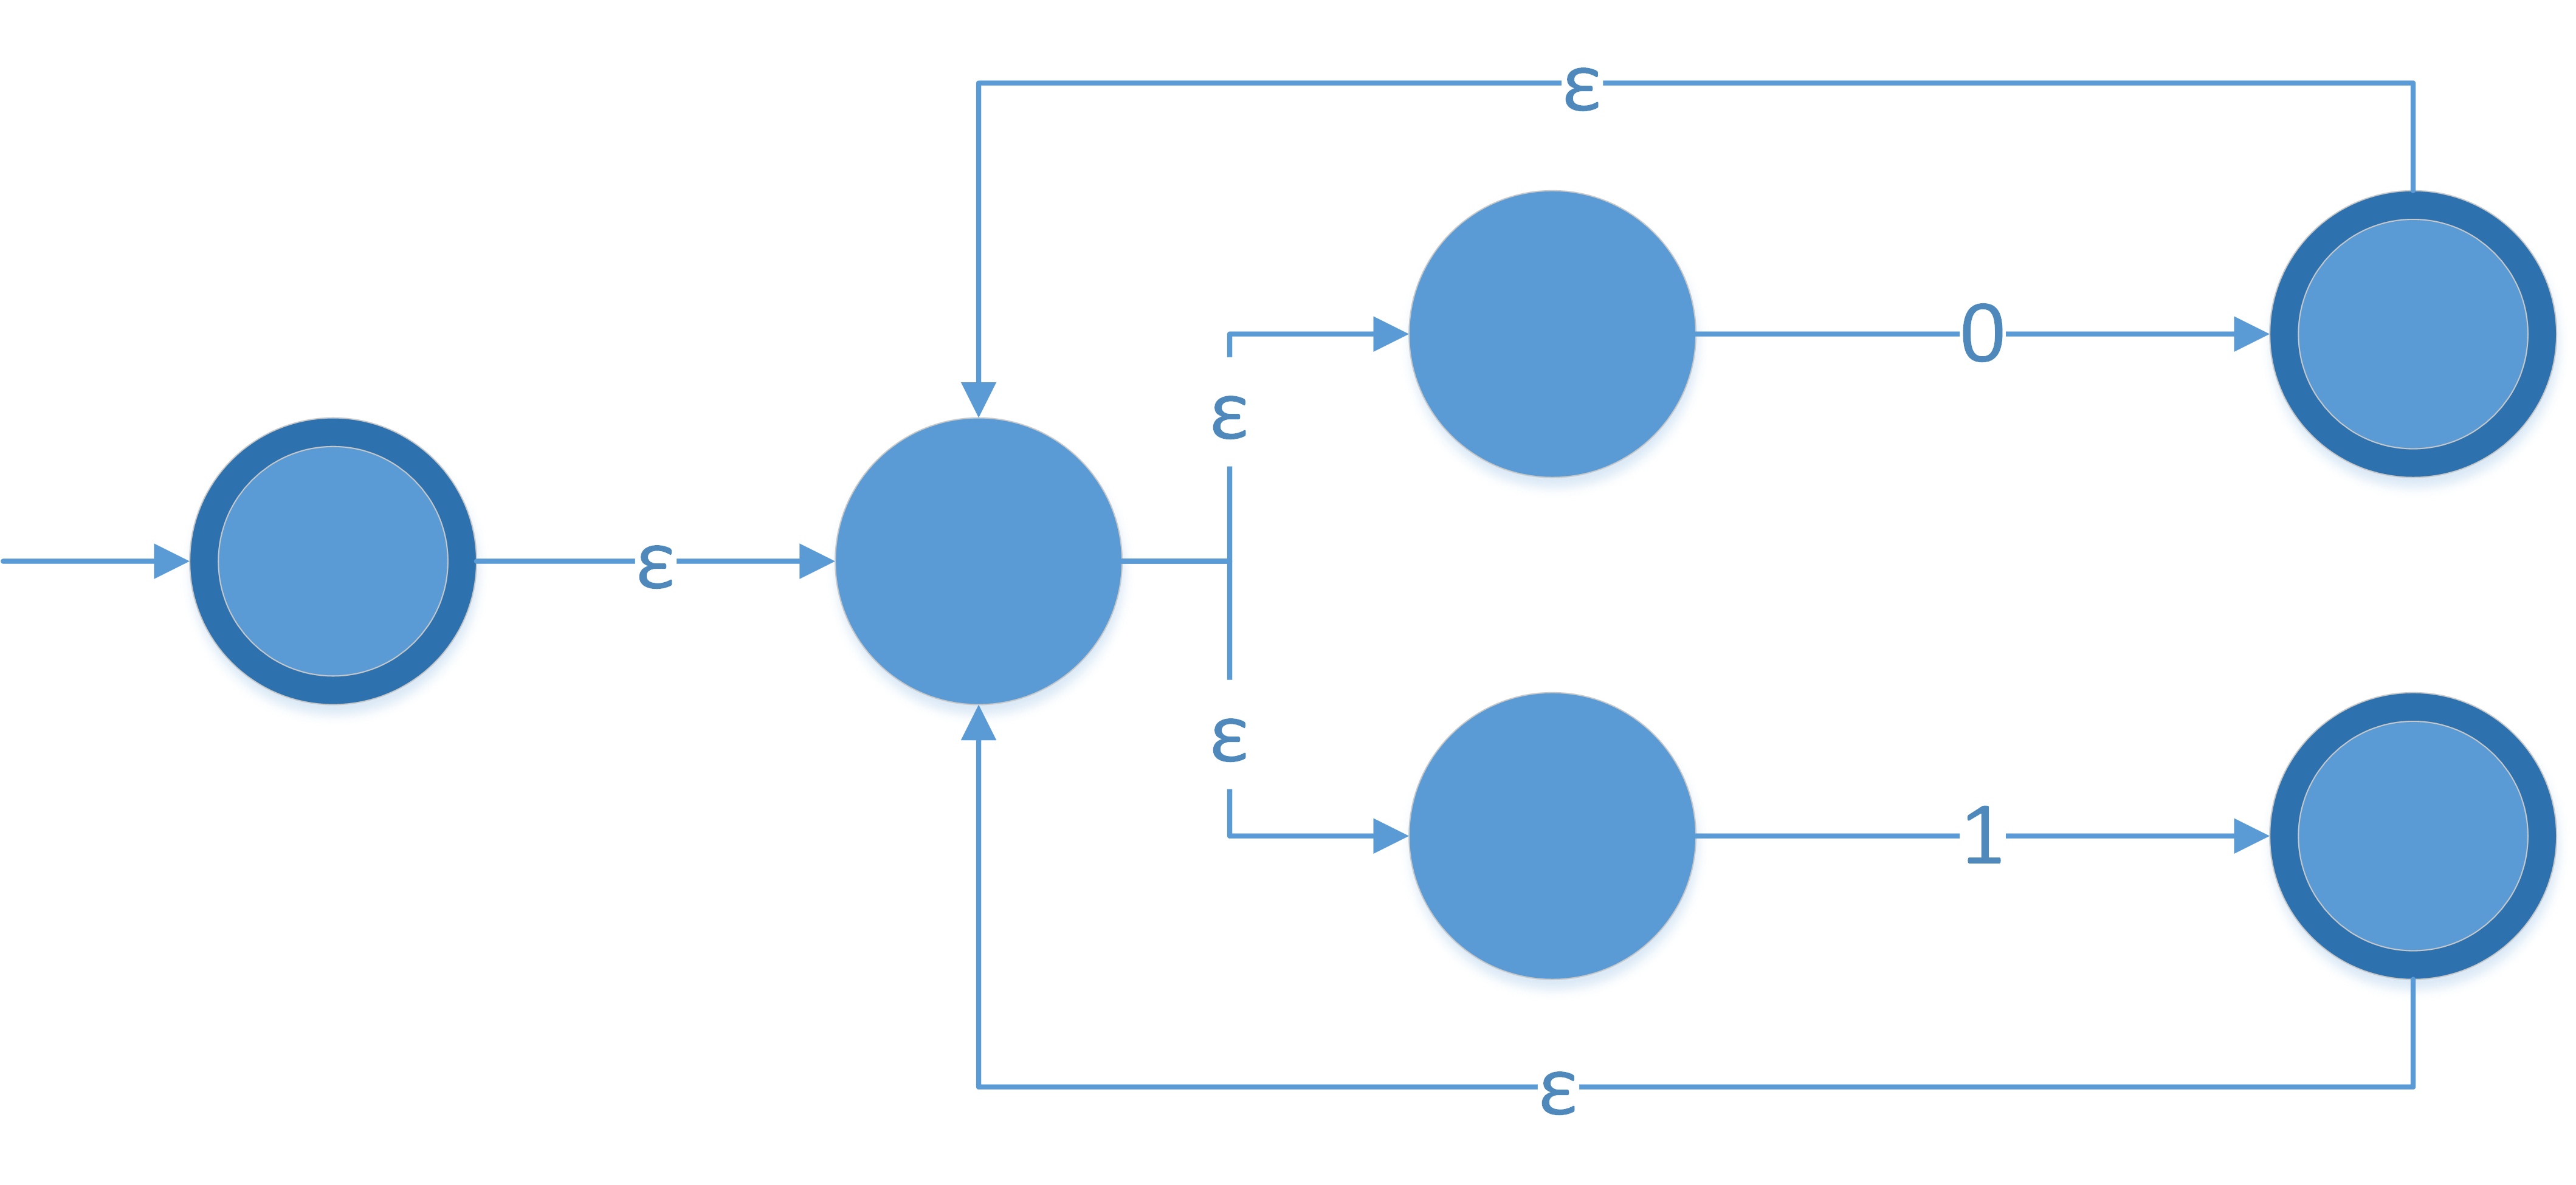
\includegraphics[width=\textwidth]{Fig12x.png}
} \caption{NFA for $\mathbf{(0\cup1)^*}$}
\label{fig:fig12}
\end{figure}

Herefter konstrueres NFA'en for $\mathbf{11}$ som set på Figur \ref{fig:fig13}.

\begin{figure}[H]%skal placeres rigtigt
{\centering 
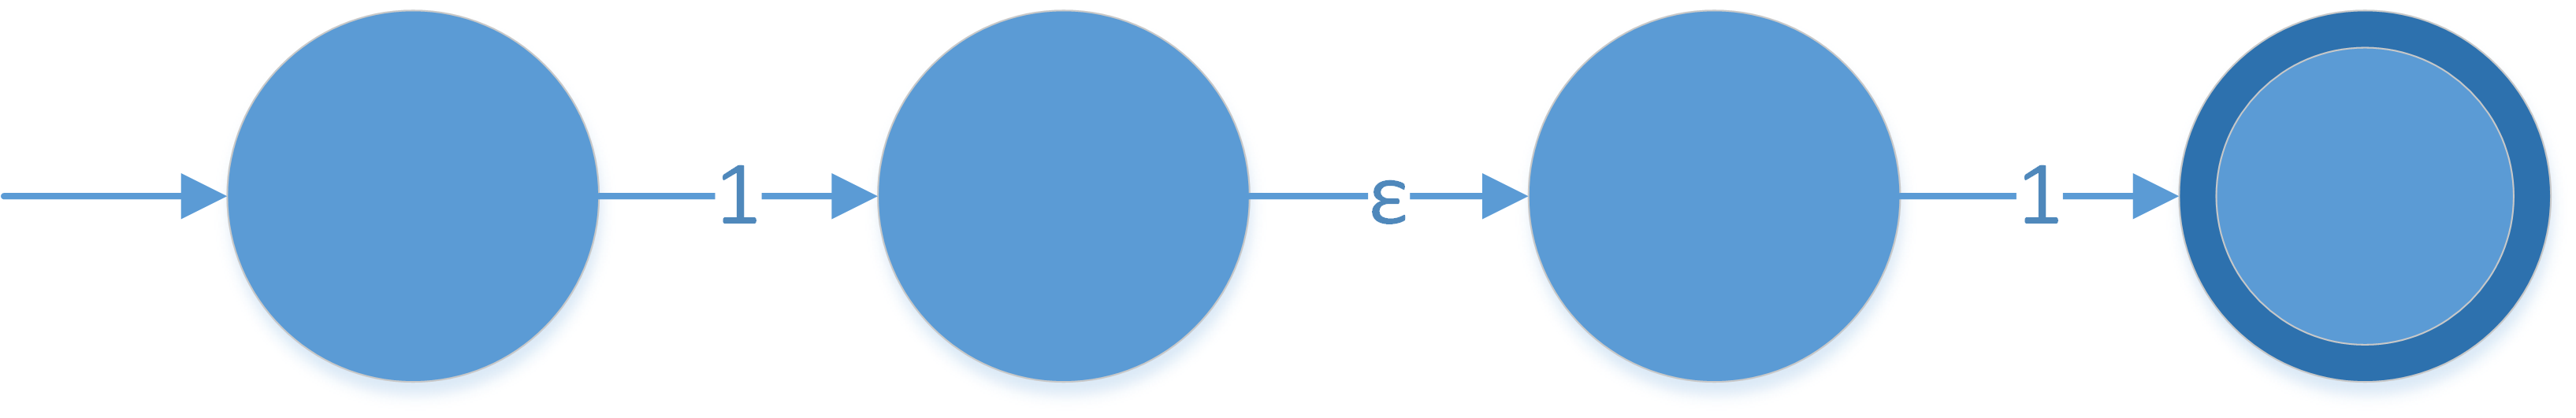
\includegraphics[width=\textwidth]{Fig13x.png}
} \caption{NFA for $\mathbf{11}$}
\label{fig:fig13}
\end{figure}

Herefter konstrueres NFA'en for $\mathbf{(0\cup1)^*11}$ som set på
Figur \ref{fig:fig14}. Denne NFA kaldes fremover $N''$.

\begin{figure}[H]%skal placeres rigtigt
{\centering 
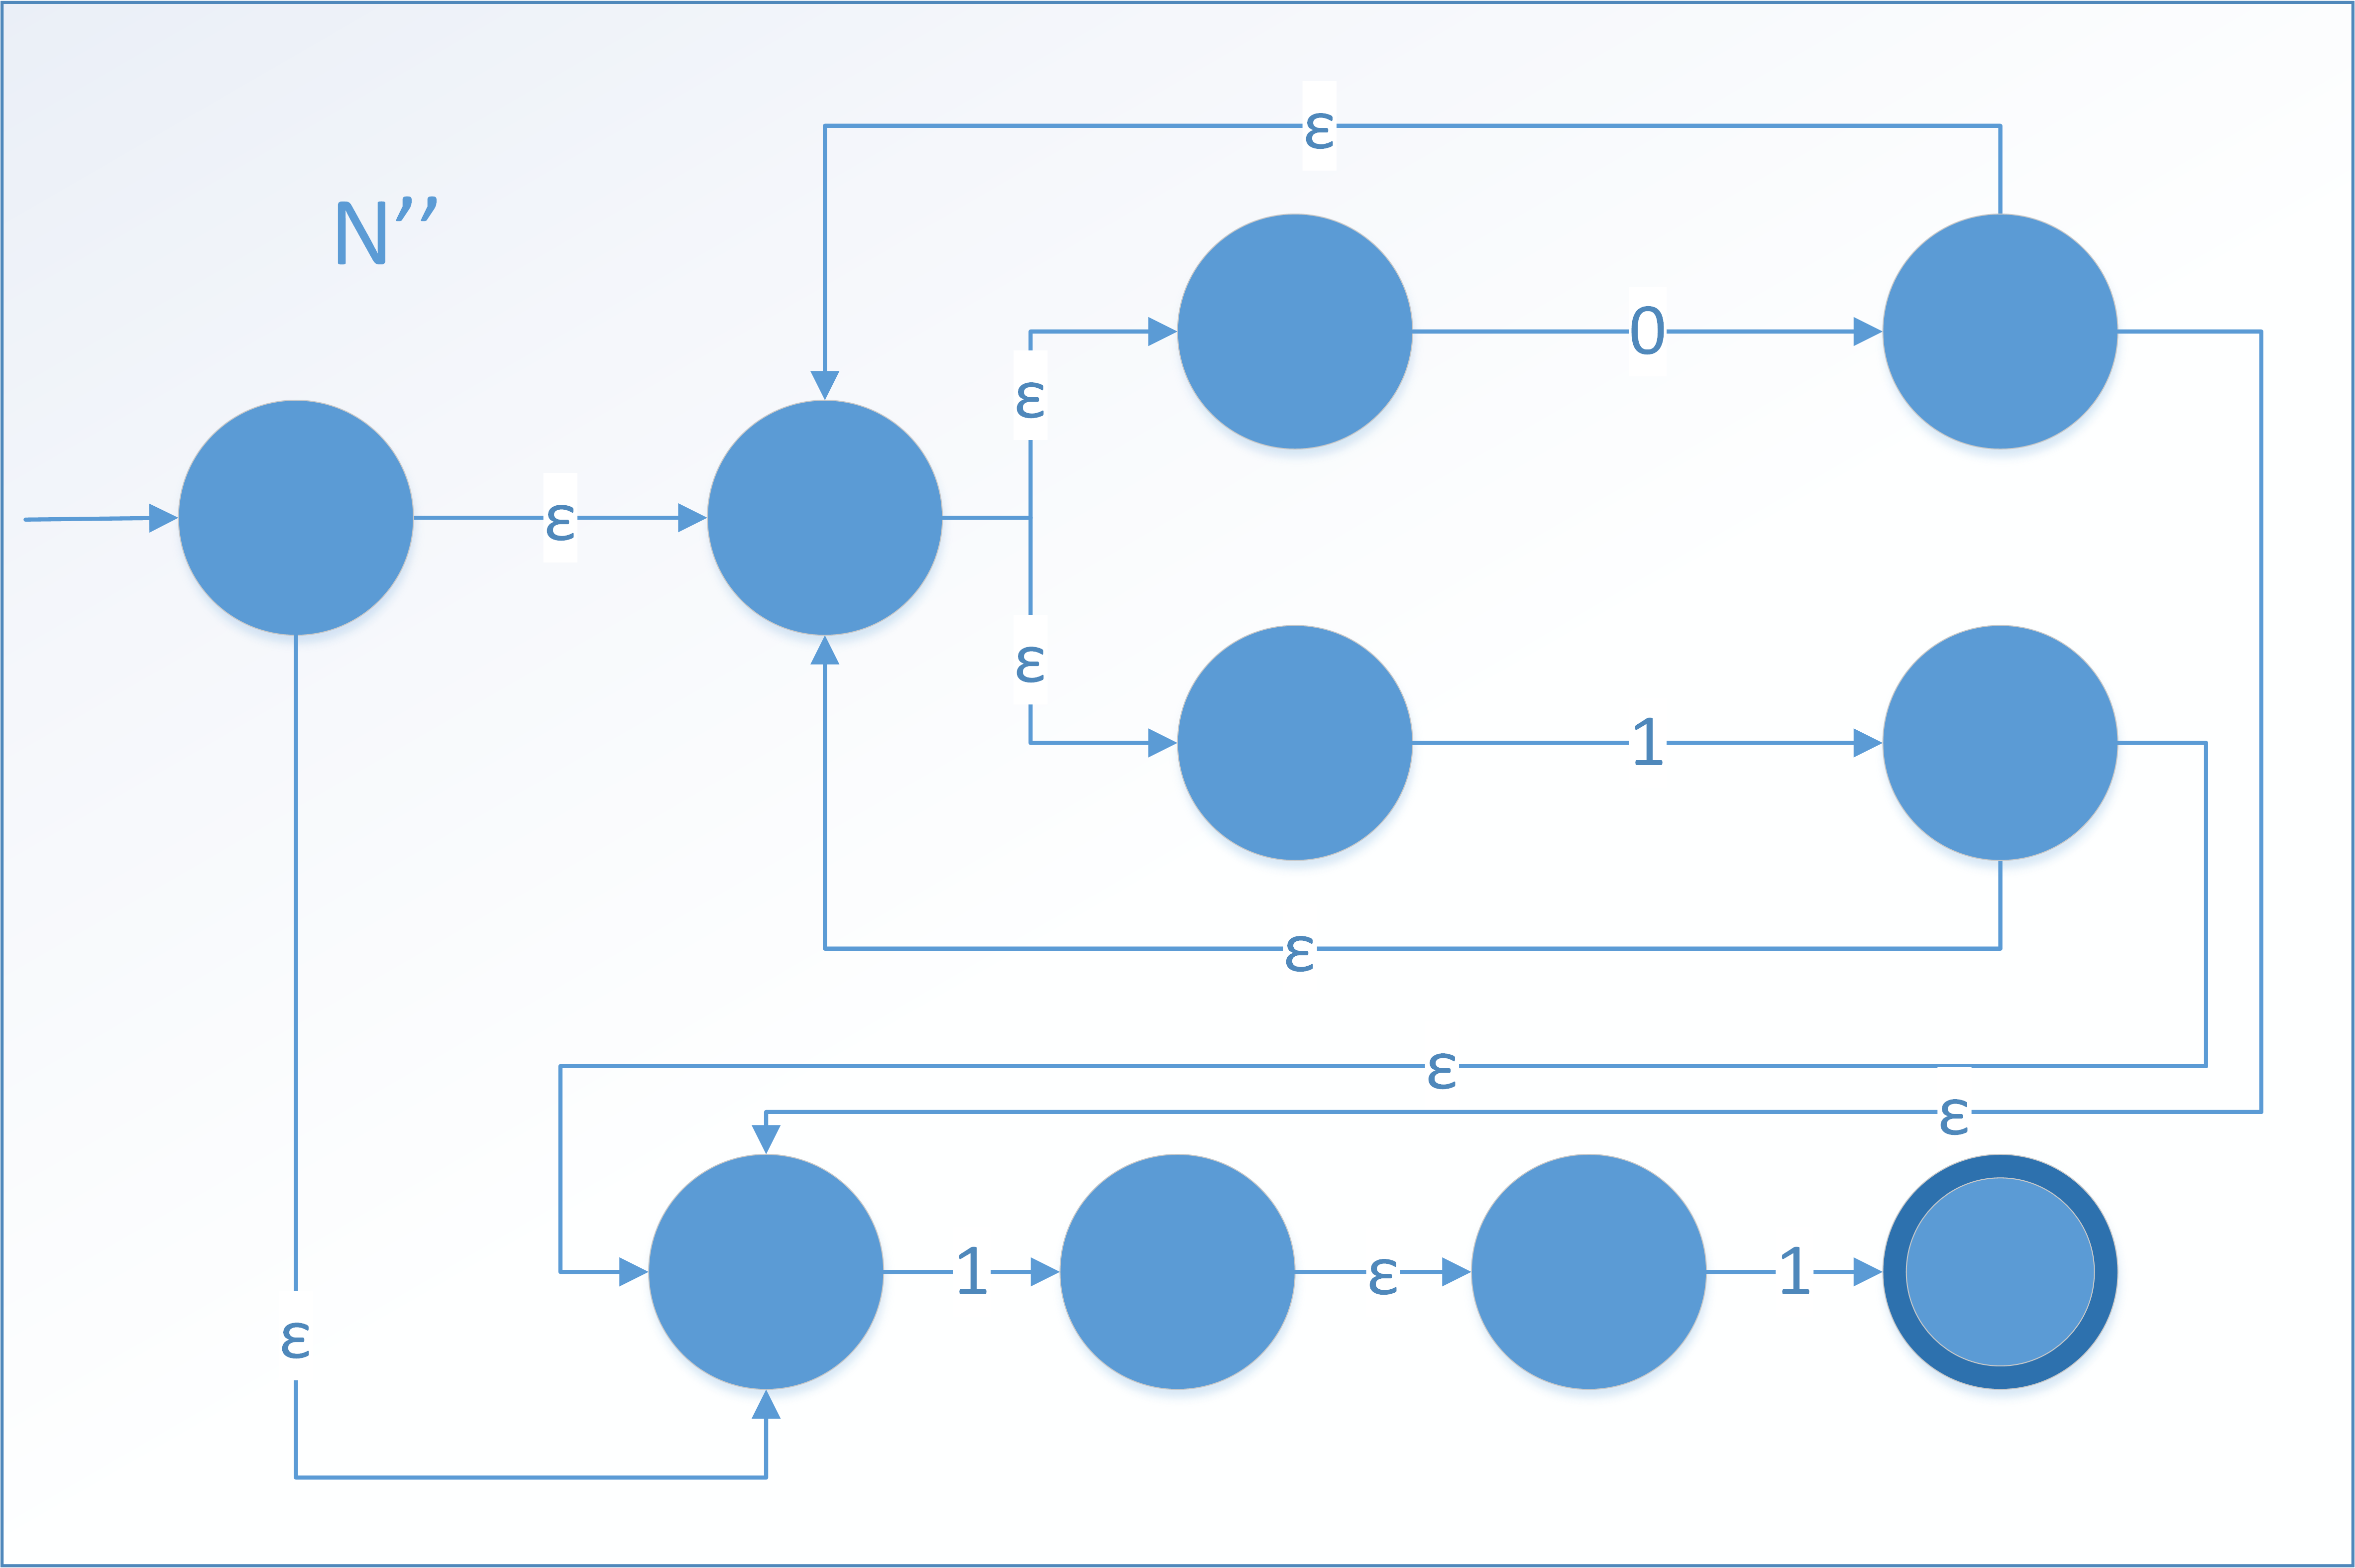
\includegraphics[width=\textwidth]{Fig14x.png}
} \caption{NFA for $\mathbf{(0\cup1)^*11}$}
\label{fig:fig14}
\end{figure}

Til slut sammensættes $N'$ og $N''$ som set på Figur \ref{fig:fig15}.

\begin{figure}[H]%skal placeres rigtigt
{\centering 
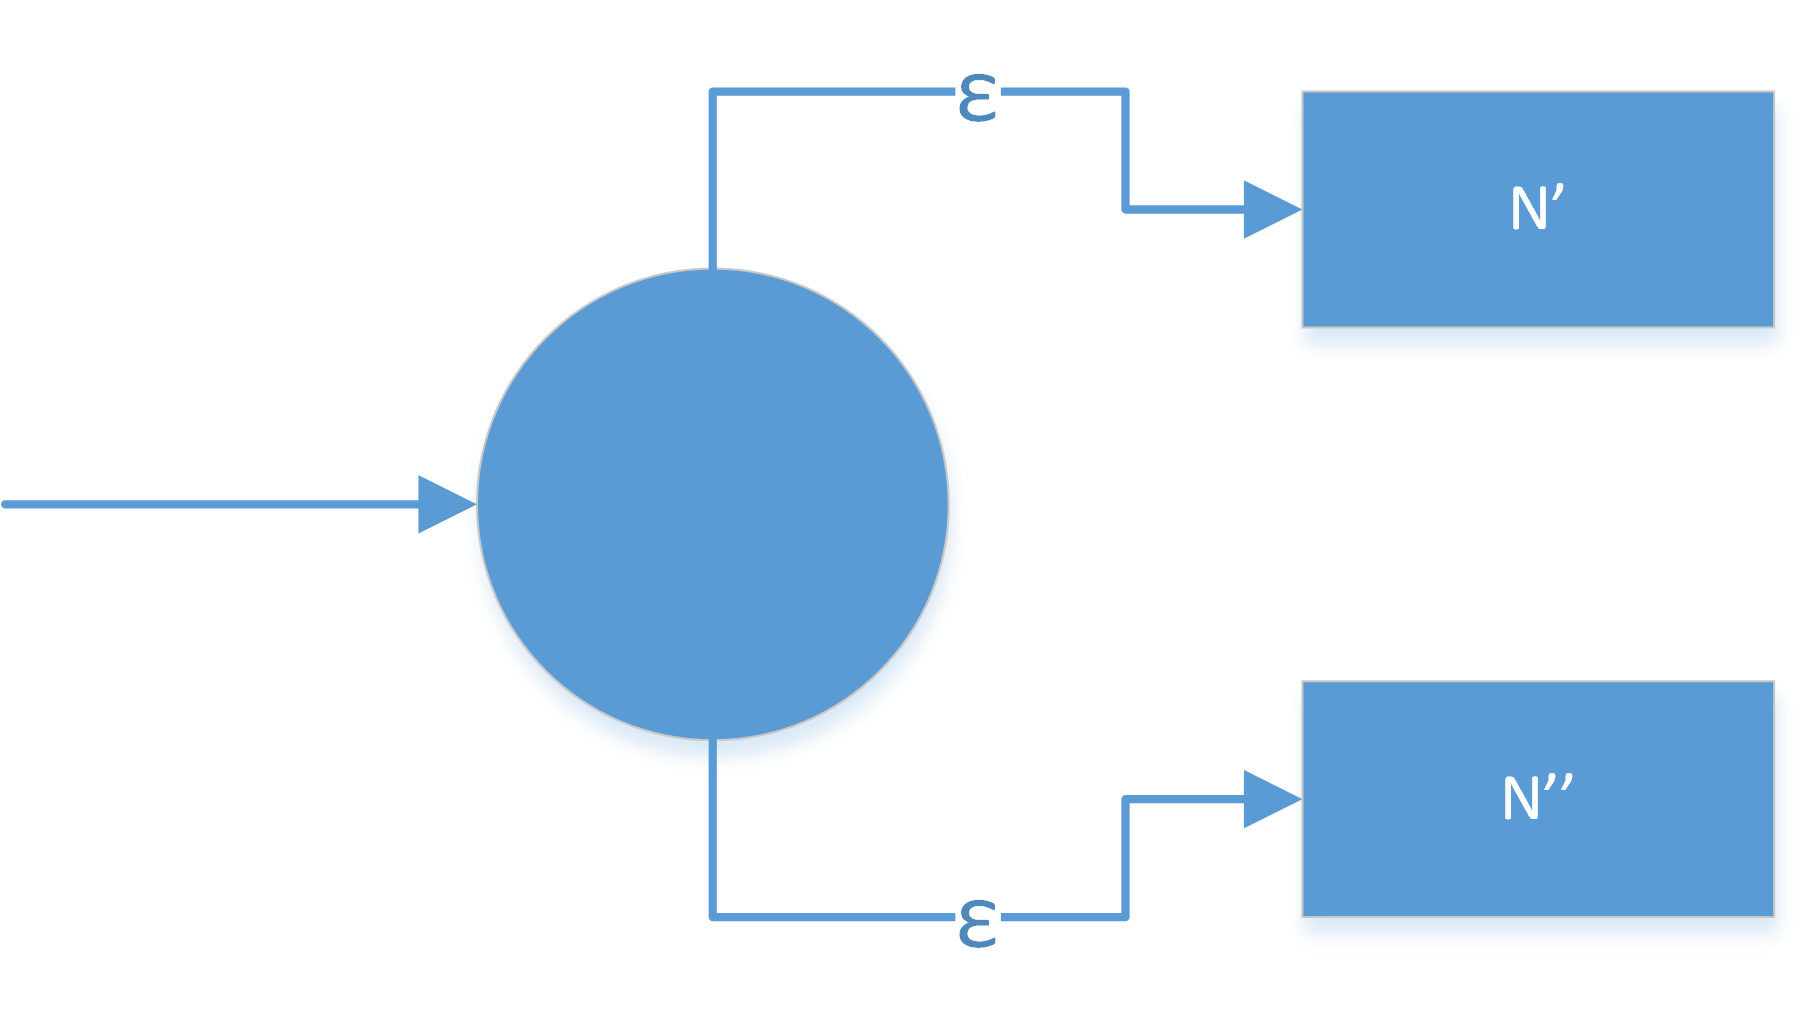
\includegraphics[width=\textwidth]{Fig15x.png}
} \caption{NFA for $\mathbf{1^*0(1^*01^*01^*)^*  \cup (1 \cup 0)^*11}$}
\label{fig:fig15}
\end{figure}
\end{eksempel}

\chapter{Fra DFA til regulære udtryk}

\begin{saetning}\label{saet:gnfa}
For enhver DFA $M$ findes der et regulært udtryk $R$ så $L(R)=L(M)$.
\end{saetning}

Bevisideen er denne:

For $M$:
\begin{itemize}
\item Lav $M$ om til en automat med regulære udtryk på transitionerne, $G_M$.
\item Fjern tilstande fra $G_M$ en ad gangen (men sådan at samme sprog genkendes).
\item Til sidst er der en en start og en sluttilstand, med et regulært udtryk på transitionen fra start til slut.
\end{itemize}

En automat med regulære udtryk på transitionerne kaldes en
\emph{generaliseret NFA} (GNFA).

\begin{definition}
En GNFA er en 5-tupel $(Q, \Sigma, q_{start}, q_{accept}, \delta)$ hvor der står regulære udtryk på transitionerne (se Figur \ref{fig:fig16}).
\end{definition}
\begin{figure}[H]%skal placeres rigtigt
{\centering 
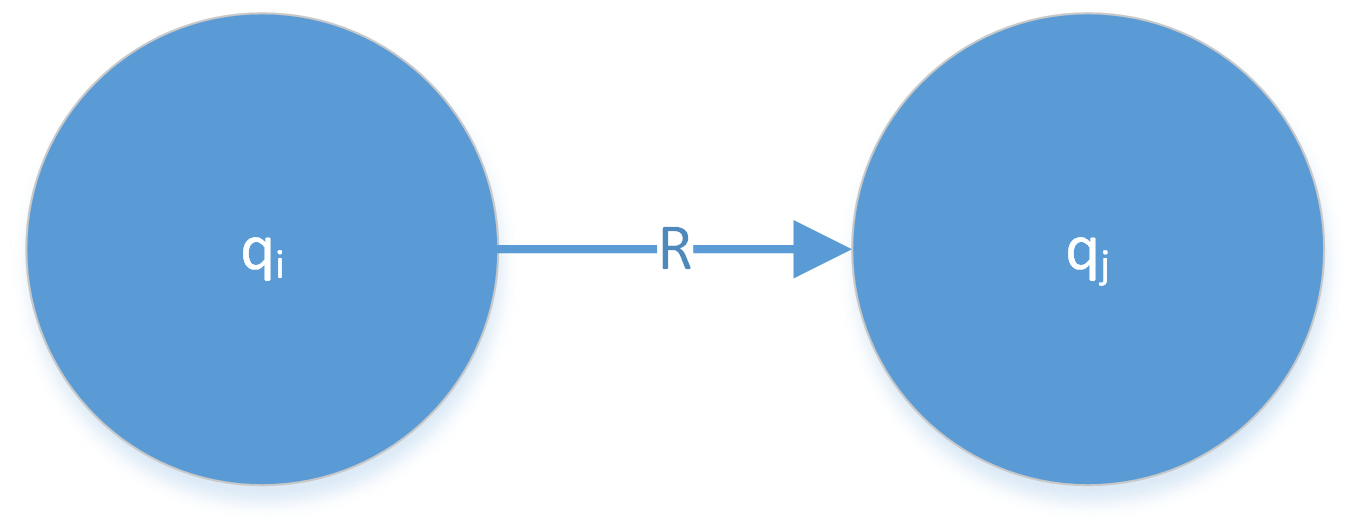
\includegraphics[width=\textwidth]{Fig16x.png}
} \caption{En GNFA med regulære udtryk på transitionerne}
\label{fig:fig16}
\end{figure}

Overføringsfunktion fortæller for hvert par af tilstande hvilket
regulært udtryk der er på transitionen mellem dem, dvs.
%
\[ \delta: Q\setminus\{q_{accept}\}\times Q\setminus\{q_{start}\} \ra
\mathcal{R} \]
%
hvor $\mathcal{R}$ betegner mængden af regulære udtryk.

En GNFA overholder denne bordskik:
\begin{enumerate}
\item En transition mellem hvert par af tilstande, dog skal det gælde
  at
\item Der er ingen transitioner \emph{fra} $q_{accept}$
\item Der er ingen transitioner \emph{til} $q_{start}$
\end{enumerate}
%
En GNFA accepterer en streng $w$ hvis $w = s_1 \ldots s_n$ og der er en
følge af tilstande $r_1 \ldots r_n$ så:
\begin{itemize}
\item $r_1 = q_{start}$
\item For alle $r_i (1 \leq i < n)$ gælder $\delta (r_i, r_{i+1})=R_i$ og $s_i \in L(R_i)$
\item $r_n = q_{accept}$
\end{itemize}

\begin{eksempel}
På Figur \ref{fig:fig17} ses et eksempel på en GNFA.

\begin{figure}[H]%skal placeres rigtigt
{\centering 
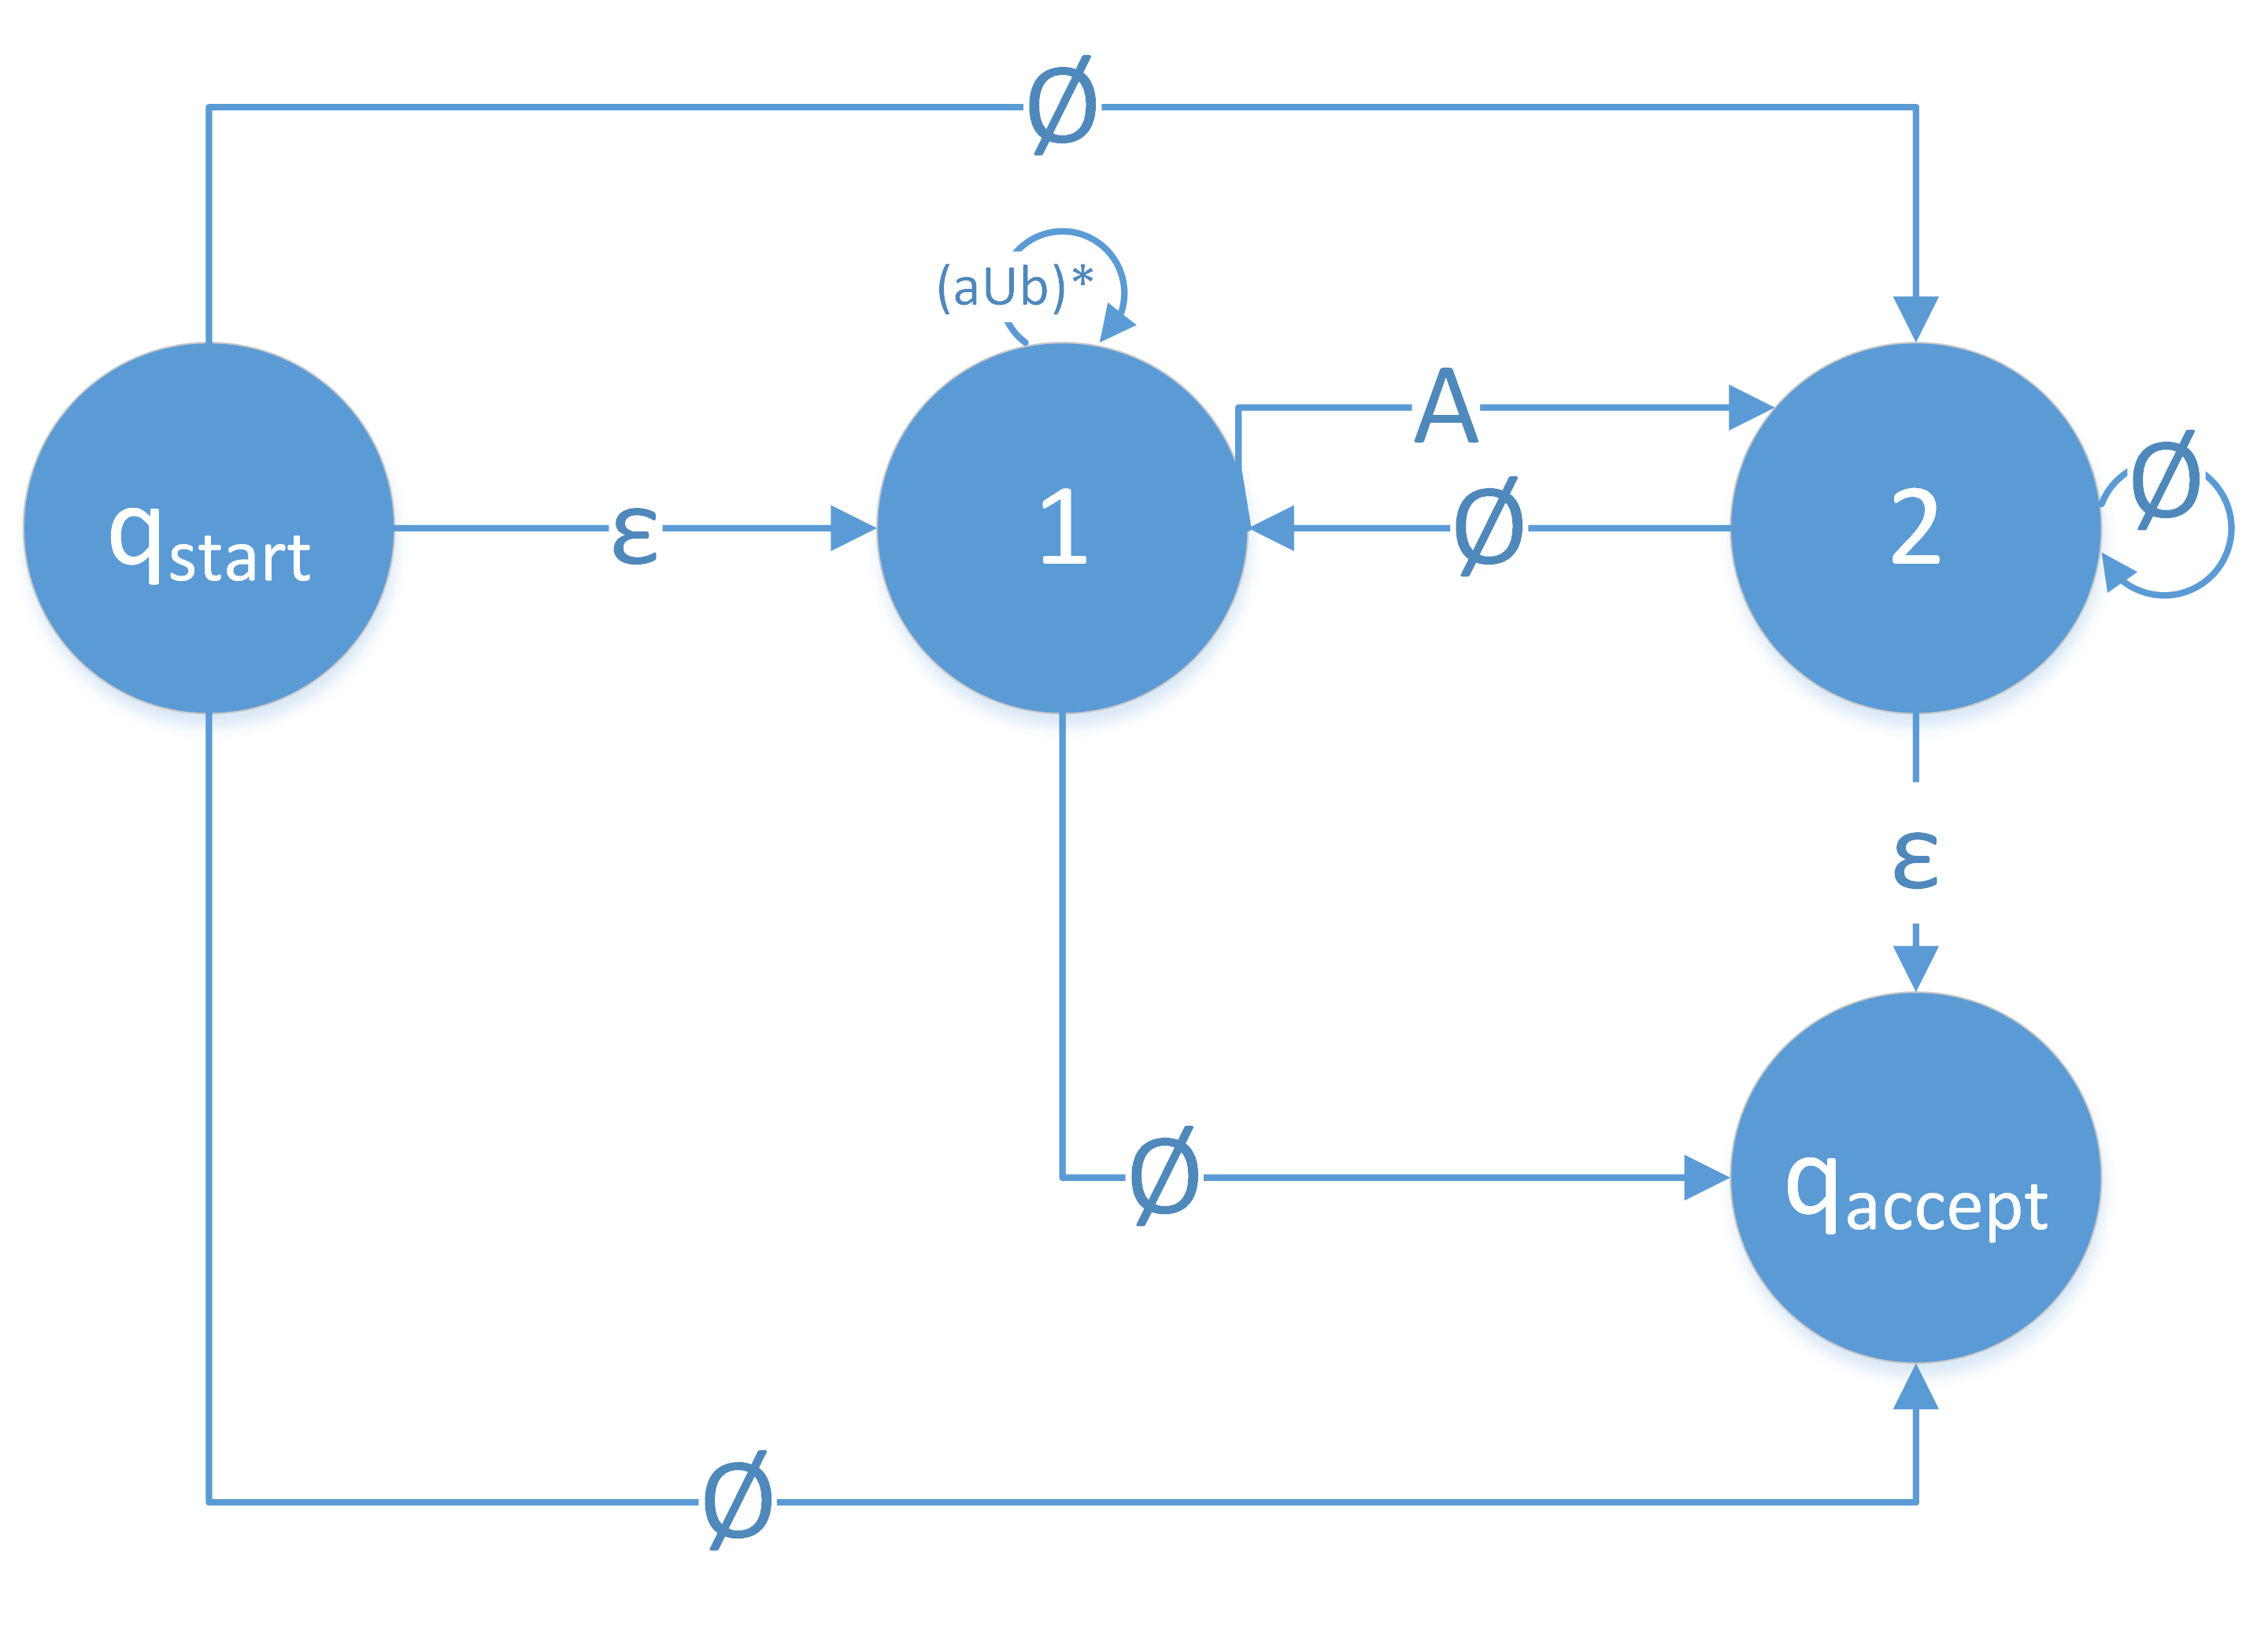
\includegraphics[width=\textwidth]{Fig17x.png}
} \caption{Et eksempel på en GNFA}
\label{fig:fig17}
\end{figure}

Her accepteres fx strengen $aaba$. Dette kan vises ved at $aaba$ kan
deles op i $\epsilon \; a a b \; a \; \epsilon$, se Figur
\ref{fig:fig18}.

\begin{figure}[H]%skal placeres rigtigt
{\centering 
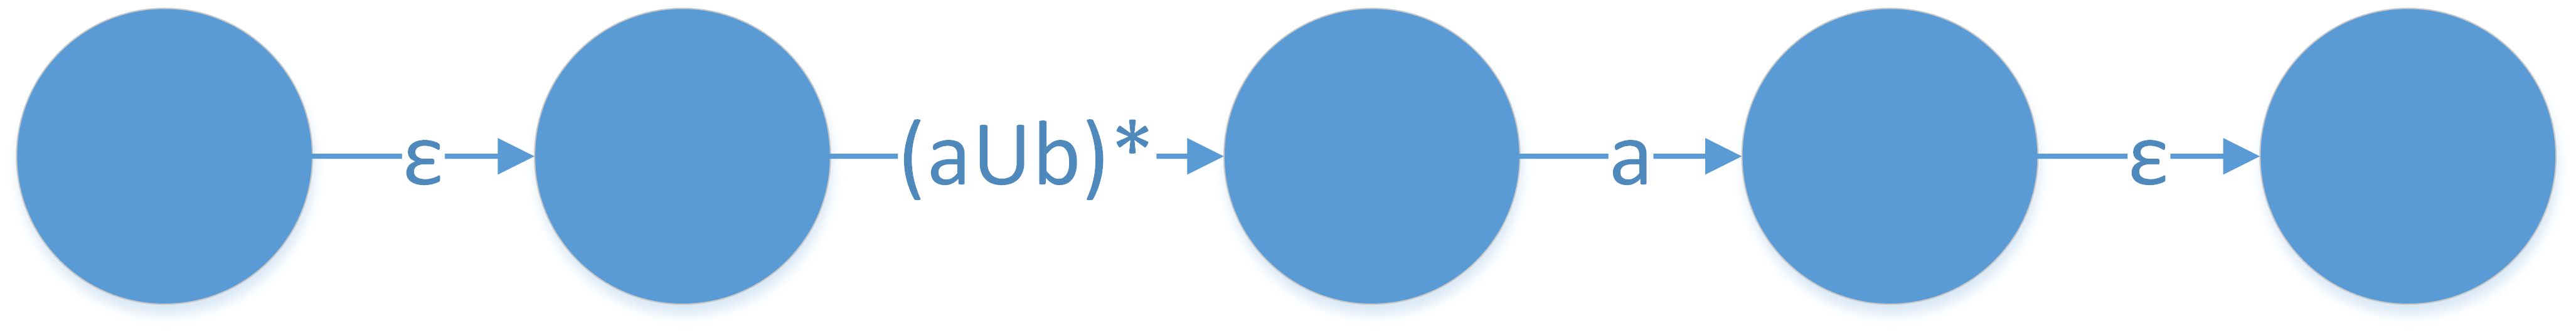
\includegraphics[width=\textwidth]{Fig18x.png}
} \caption{Sådan kan strengen $aaba$ læses af GNFA'en fra Figur
  \ref{fig:fig17}}
\label{fig:fig18}
\end{figure}
\end{eksempel}

\begin{bevis}(for Sætning \ref{saet:gnfa})
Givet en DFA $M$ der ønsket skrevet i form at regulære udtryk.
Først skal $M$ laves om til en GNFA.
Dette gøres ved:
\begin{itemize}
\item Indfør ny $q_{start}$ og en transition $\epsilon$ til det gamle startpunkt ved $M$
\item Indfør ny $q_{accept}$ og lav for hver gammen accepttilstand en $\epsilon$ transition til $q_{accept}$
\item Hvis der ikke er en transition mellem $q_i$ og $q_j$ i M tilføjes en transition mærket $\emptyset$
\item Saml transitioner med $\cup$ så en transition mærket $a,b$ i stedet bliver mærket $a\cup b$
\end{itemize}

Herefter fjernes tilstandene en efter en, så der kun er $q_{start}$ og
$q_{accept}$ tilbage.  Hver gang en tilstand fjernes fra $M$ og vi får
en ny automat $M'$, skal vi sikre at $L(M') = L(M)$, dvs. at vores nye
automat genkender samme sprog som den gamle.

Dette gør vi således. Lad $q_{rip}$ være den tilstand som vi
fjerner. Det skal gælde at $q_{rip} \neq q_{start}$ og $q_{rip} \neq
q_{accept}$. 

Da vores GNFA $M$ overholder bordskik, er der en transition mellem
hvert par af tilstande. Betragt to vilkårlige tilstande
$q_i,q_j$ som også skal findes i $M'$. På grund af vores krav om
bordskik ved vi at der er
%
\begin{itemize}
\item en transition fra $q_i$ til $q_j$ mærket med $R_4$
\item en transition fra $q_i$ til $q_{rip}$ mærket med $R_1$
\item en transition fra $q_{rip}$ til $q_{rip}$ mærket med $R_2$
\item en transition fra $q_{rip}$ til $q_j$ mærket med $R_3$
\end{itemize}
%
Hvad for et regulært udtryk skal der stå på transitionen i $M'$ fra
$q_i$ til $q_J$? Der skal stå et regulært udtryk der beskriver alle de
strenge, der kan føre os fra $q_I$ til $q_j$. Dette regulære udtryk er
%
\[  R_4 \cup R_1(R_2)^* R_3 \]
%
Dette kan ses på Figur \ref{fig:fig19}. Bemærk at dette skal gøres
\emph{for hvert par af tilstande $q_i,q_j$}, herunder i tilfældene
hvor $q_i = q_j$ (der skal være en tilstand mellem hvert par af
tilstande, herunder fra hver tilstand, der ikke er $q_{start}$ eller
$q_{accept}$, til sig selv).

\begin{figure}[H]%skal placeres rigtigt
{\centering 
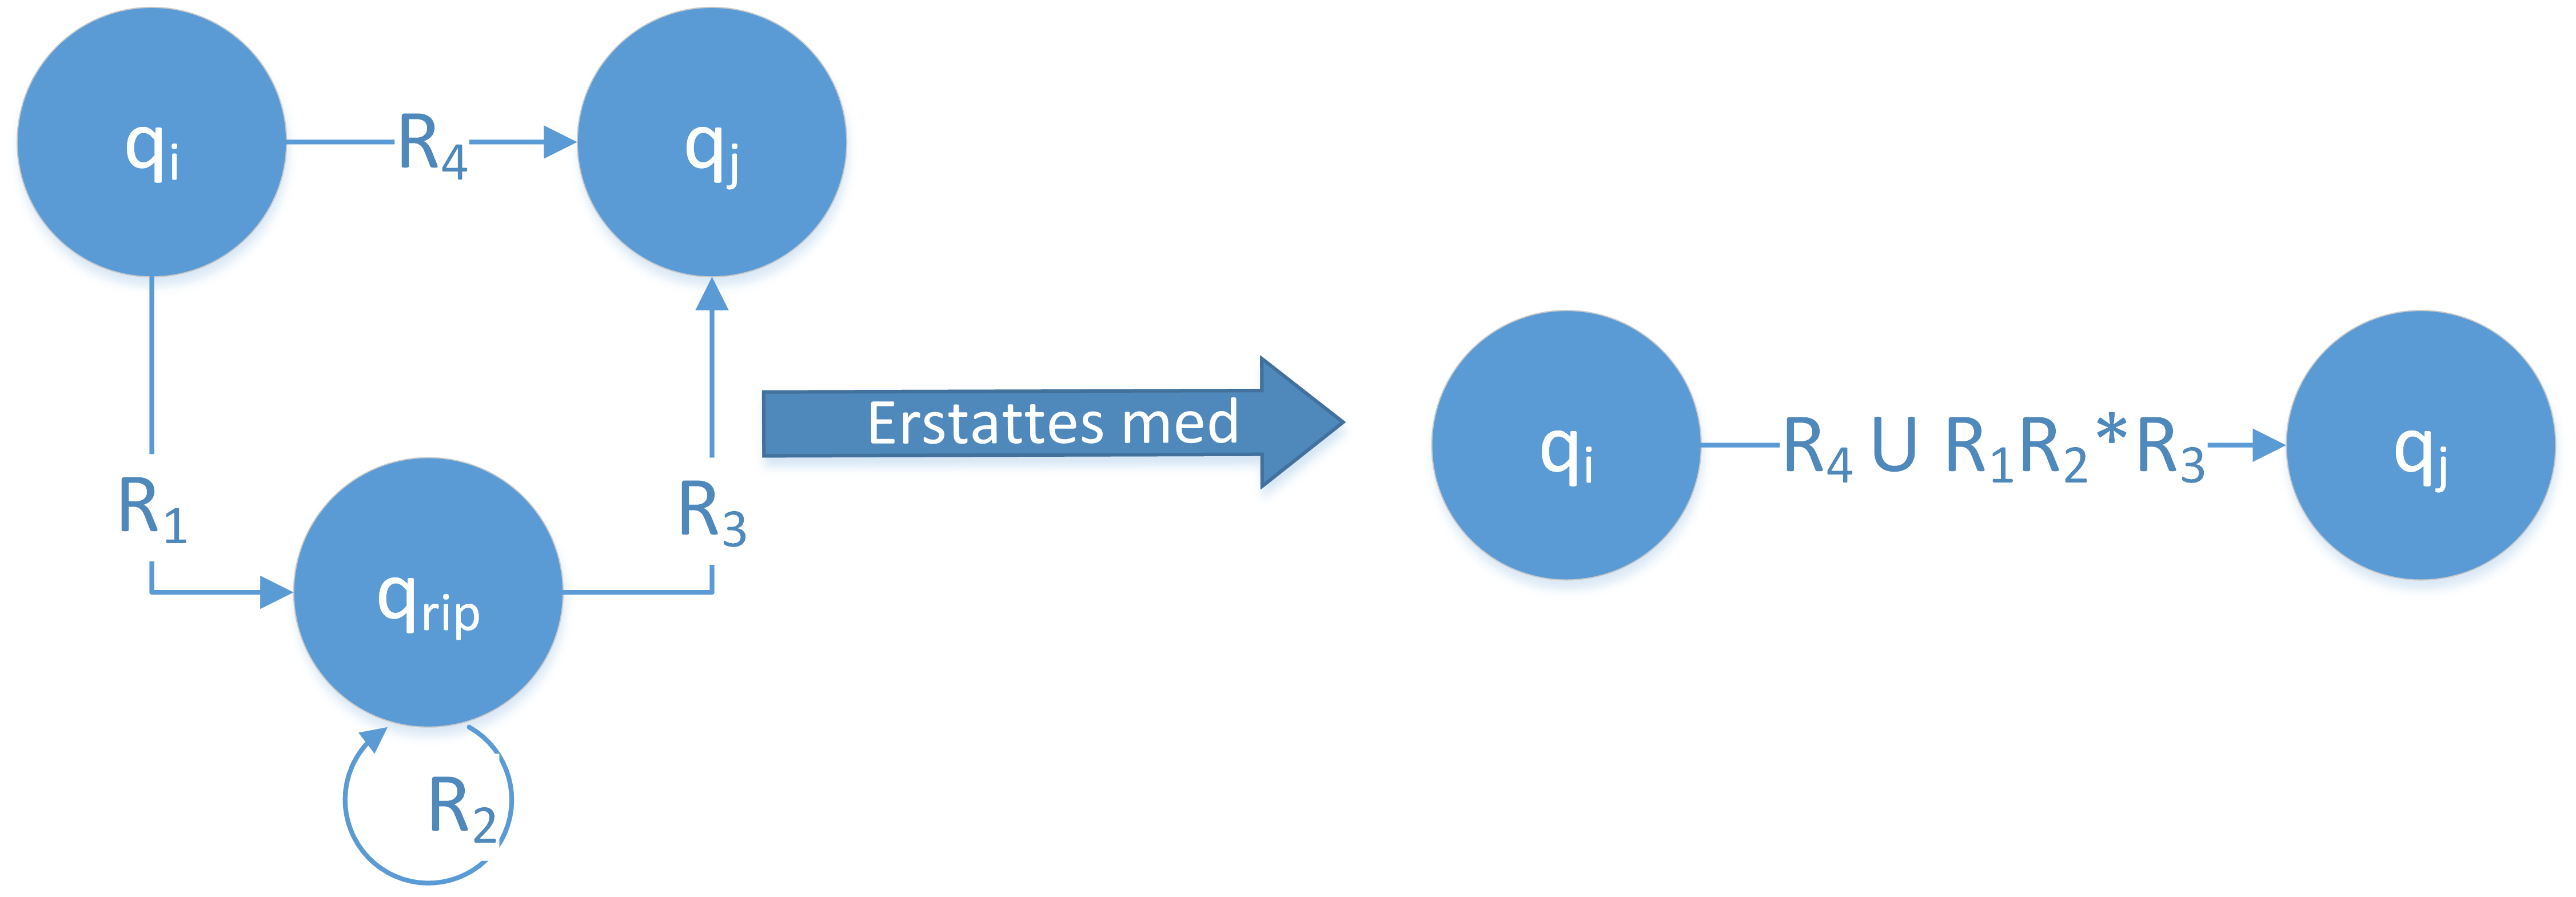
\includegraphics[width=\textwidth]{Fig19x.png}
} \caption{Sådan laves den nye transition mellem $q_i$ og $q_j$}
\label{fig:fig19}
\end{figure}

Den samlede konverteringsalgoritme er

\begin{quote}
\noindent $\textit{CONVERT}(G) = $
\begin{enumerate}
\item Lad $Q_G$ betegne mængden af tilstande i $G$. Hvis de eneste
  tilstande i $Q_G$ er $q_{start}$ og $q_{accept}$, så returnér det
  regulære udtryk på transitionen mellem $q_{start}$ og $q_{accept}$.
\item Ellers vælg en tilstand $q_{rip} \in Q_G$ hvor $q_{rip} \neq q_{start}$
  og $q_{rip} \neq q_{accept}$. Lad mængden af tilstande i den nye automat være
  $Q_G \setminus \set{q_{rip}}$.
\item For hvert par af tilstande $q_i,q_j$ skab den nye transition som
  angivet på Figur \ref{fig:fig19}.
\item Kald den nye automat for $G'$.
\item Kald $\textit{CONVERT}(G')$.
\end{enumerate}
\end{quote}
\end{bevis}

\begin{eksempel}
Givet er en DFA kaldet $M$, som kan ses på Figur \ref{fig:fig20}.
\begin{figure}[H]%skal placeres rigtigt
{\centering 
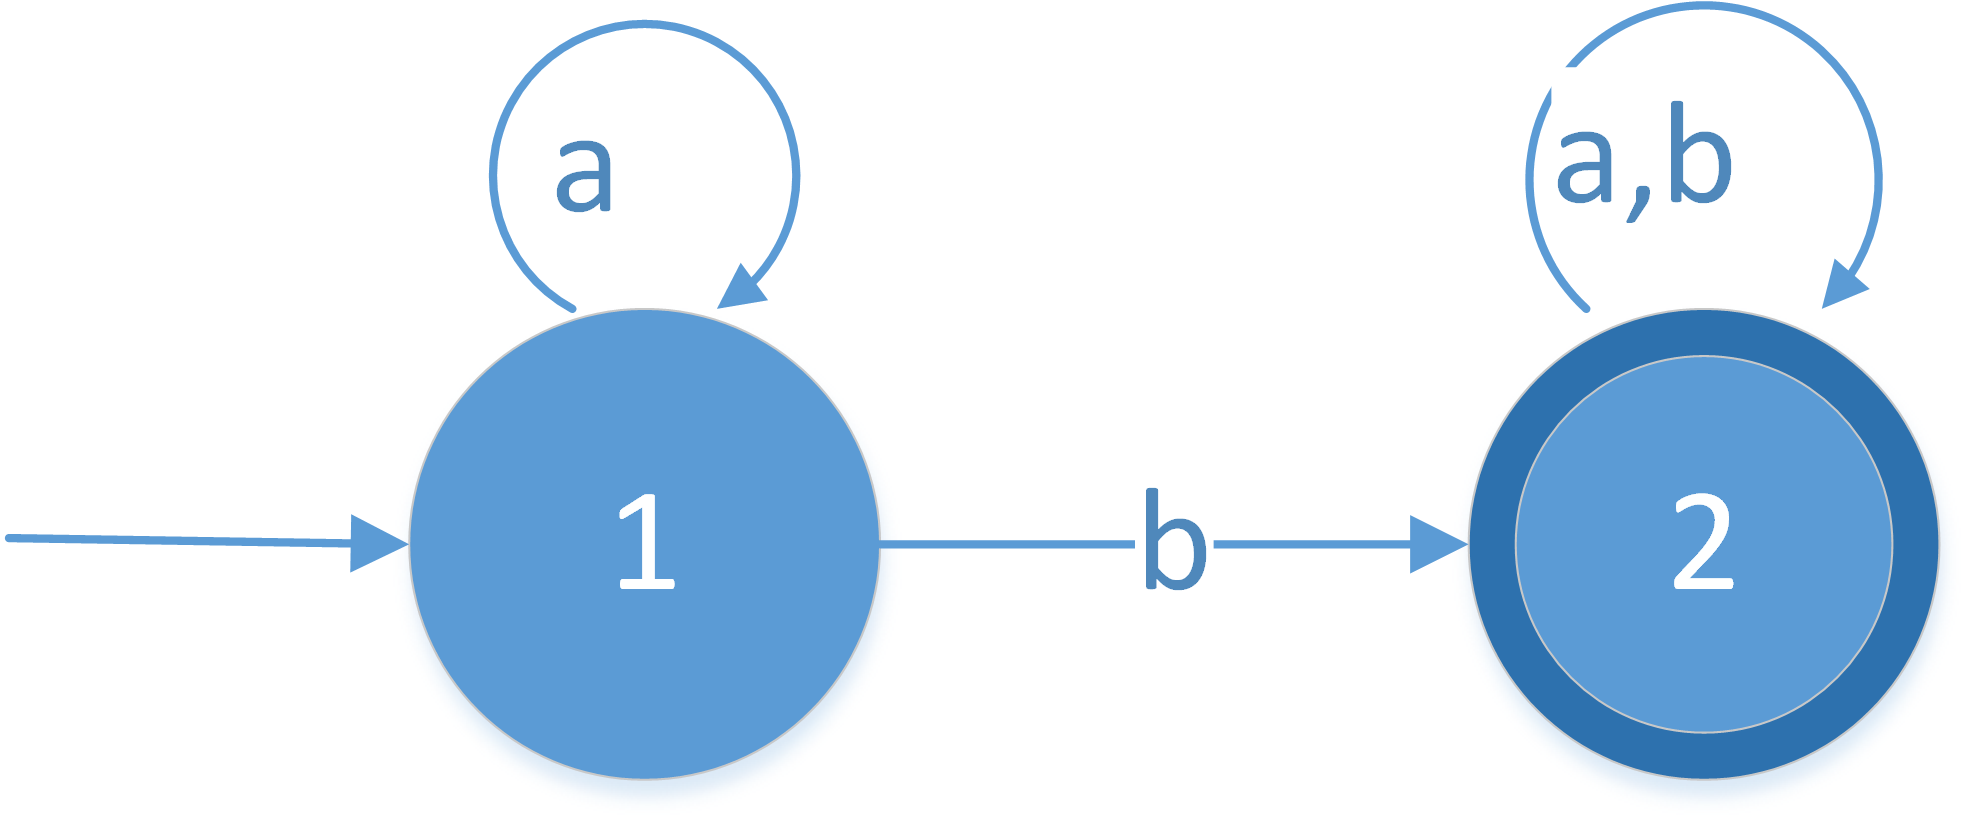
\includegraphics[width=\textwidth]{Fig20x.png}
} \caption{En DFA $M$}
\label{fig:fig20}
\end{figure}

Herefter laves en GNFA ud fra DFA'en $M$, som kan ses på Figur \ref{fig:fig21}.
\begin{figure}[H]%skal placeres rigtigt
{\centering 
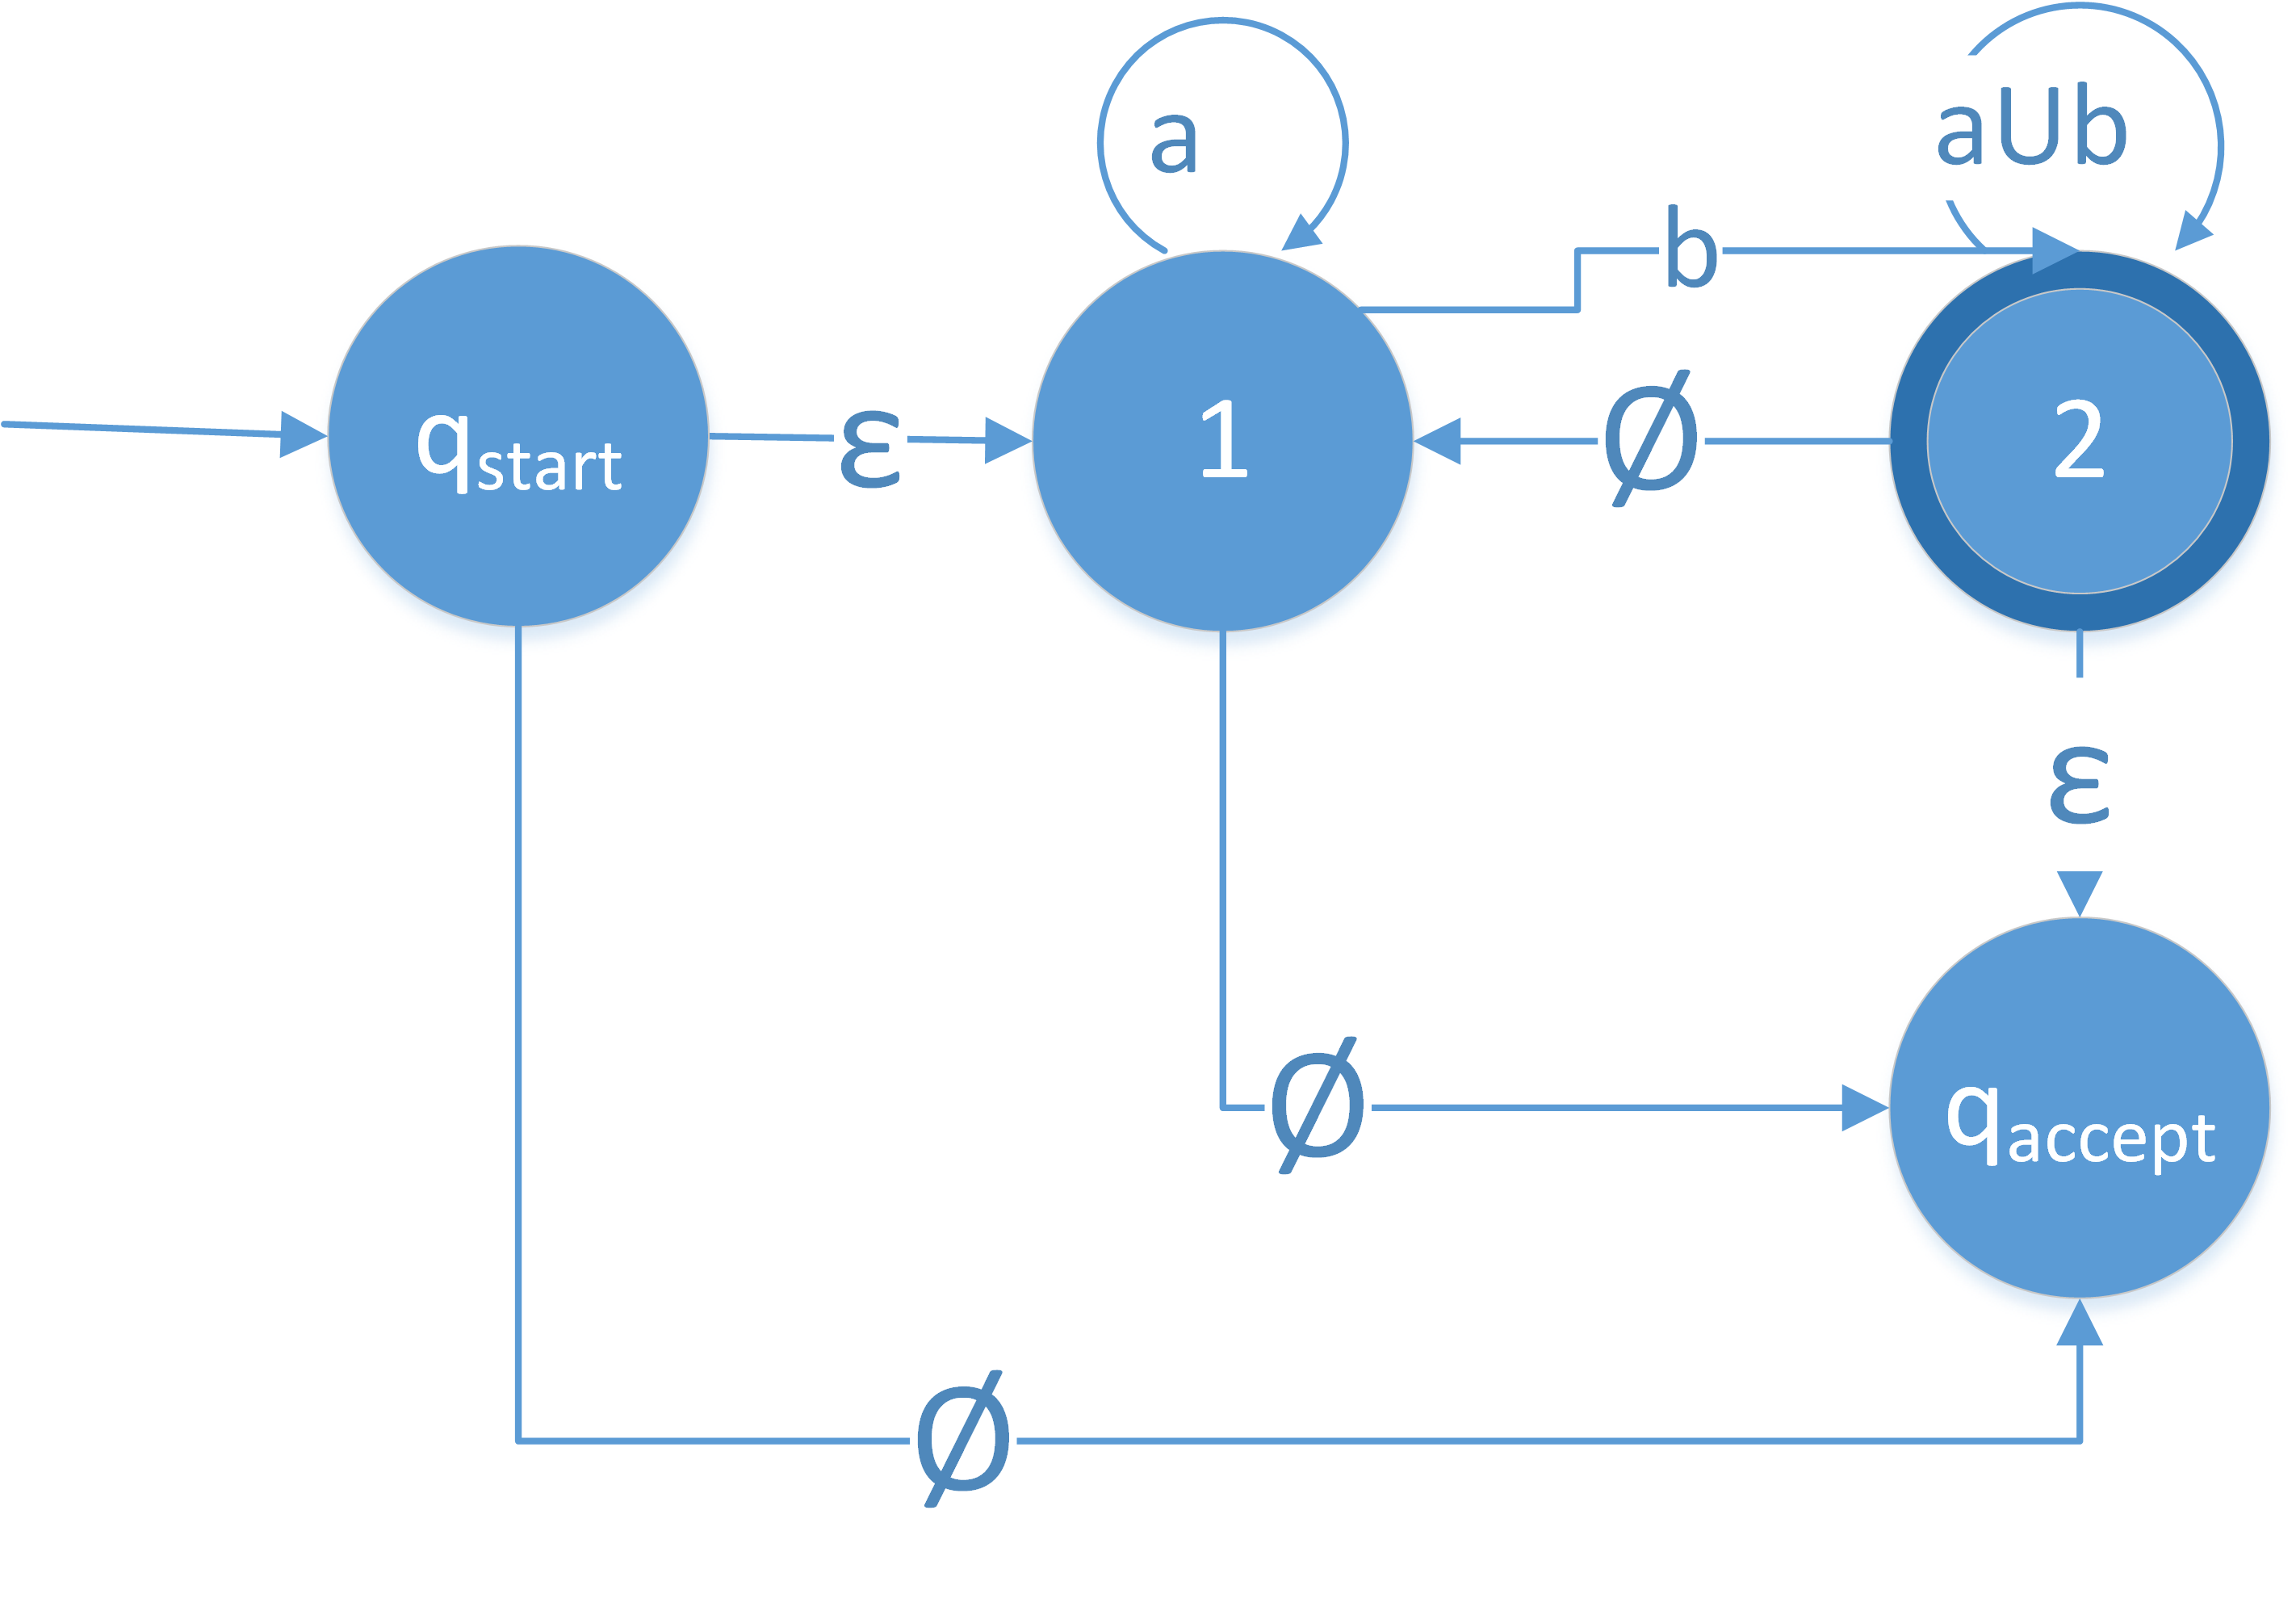
\includegraphics[width=\textwidth]{Fig21x.png}
} \caption{En GNFA ud fra DFA'en $M$}
\label{fig:fig21}
\end{figure}

Først vælges tilstand 1 som $q_{rip}$ som ses på \ref{fig:fig22}.
\begin{figure}[H]%skal placeres rigtigt
{\centering 
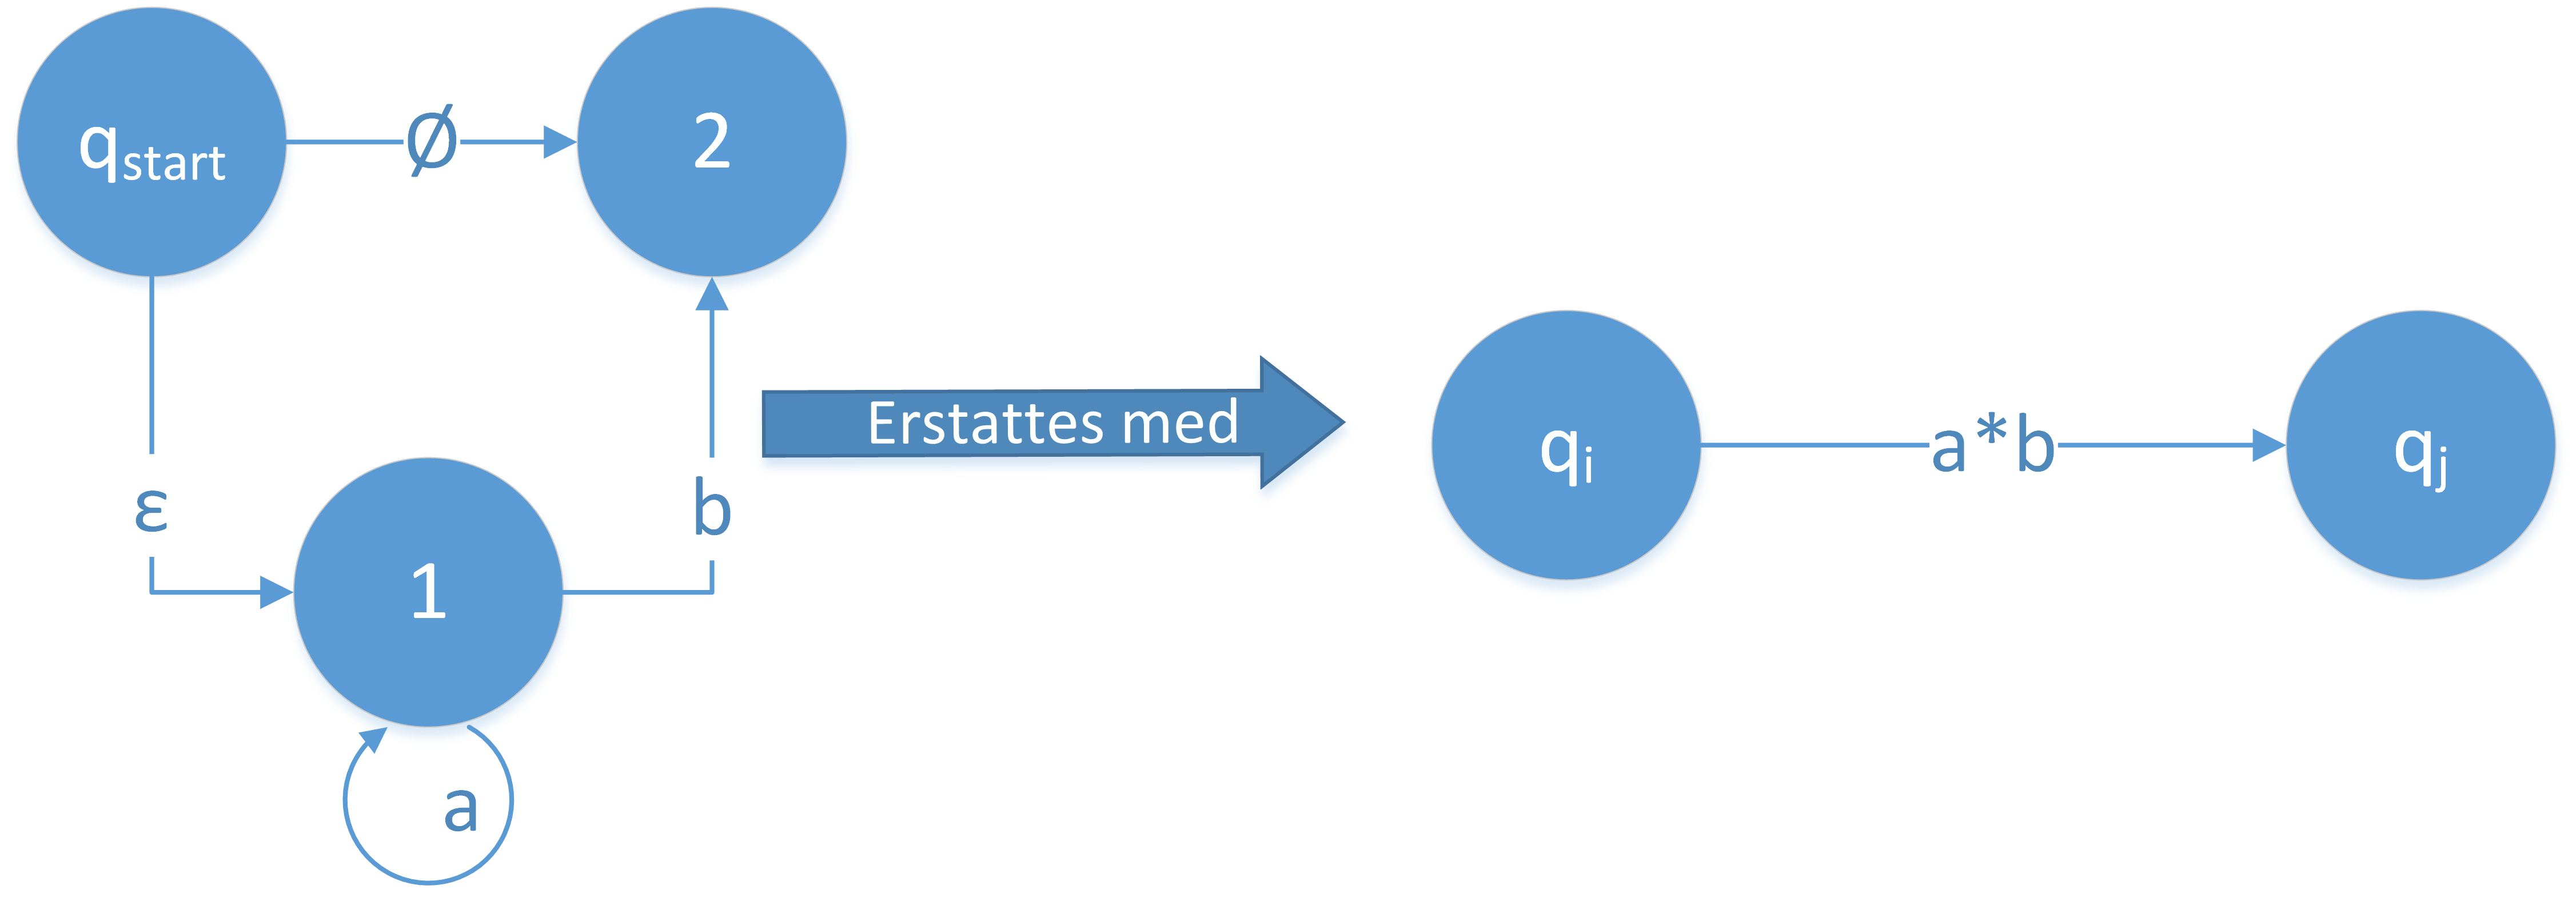
\includegraphics[width=\textwidth]{Fig22x.png}
} \caption{Udledningen af det regulære udtryk der skal erstatte tilstand
  1}
\label{fig:fig22}
\end{figure}
Dernæst vælges tilstand 2 som $q_{rip}$ og resultatet er en GNFA hvis
eneste transition er mærket med det regulære udtryk $a^*b(a\cup b)^*$.
\end{eksempel}

\chapter{Gyser}

\section{Termolig}

Forbløffende mange har problemer med terminologien også her.

\begin{itemize}
\item Regulære udtryk \emph{beskriver} sprog, automater \emph{genkender} sprog.
\begin{itemize}
\item ikke ``regulære udtryk genkender''
\item ikke ``regulære udtryk accepterer''
\end{itemize}
\end{itemize}

\section{Ingen ad-hoc-løsninger, tak!}

Nogle studerende vil af en eller anden grund ikke bruge tid på at lære
de generelle konstruktioner som dukker op i kurset. Når de til eksamen
bliver bedt om at konstruere en NFA ud fra et regulært udtryk eller
bliver bedt om at et regulært udtryk ud fra en DFA, prøver de at finde
automaten eller det regulære udtryk ved at gætte sig frem.

Men formålet med denne type opgave er \emph{at finde ud af om den
  studerende kender den generelle konstruktion}. Noget helt andet er
at de studerende, der ad hoc'er sig frem, aldrig får fundet den
rigtige automat eller det rigtige regulære udtryk!


\section{Ingen smarte genveje, tak!}

Nogle studerende tror at man kan ``spare'' ved at lade være med at
bruge de korrekte konstruktioner og gøre som f.eks. på Figur
\ref{fig:fig23}. 

Men den slags fører meget, meget let til fejl -- og man glemmer meget,
meget let hvad den generelle metode består i. Gør det rigtigt fra
starten, og undgå ``smarte genveje'' der ignorerer den generelle
metode.

\begin{figure}[H]%skal placeres rigtigt
{\centering 
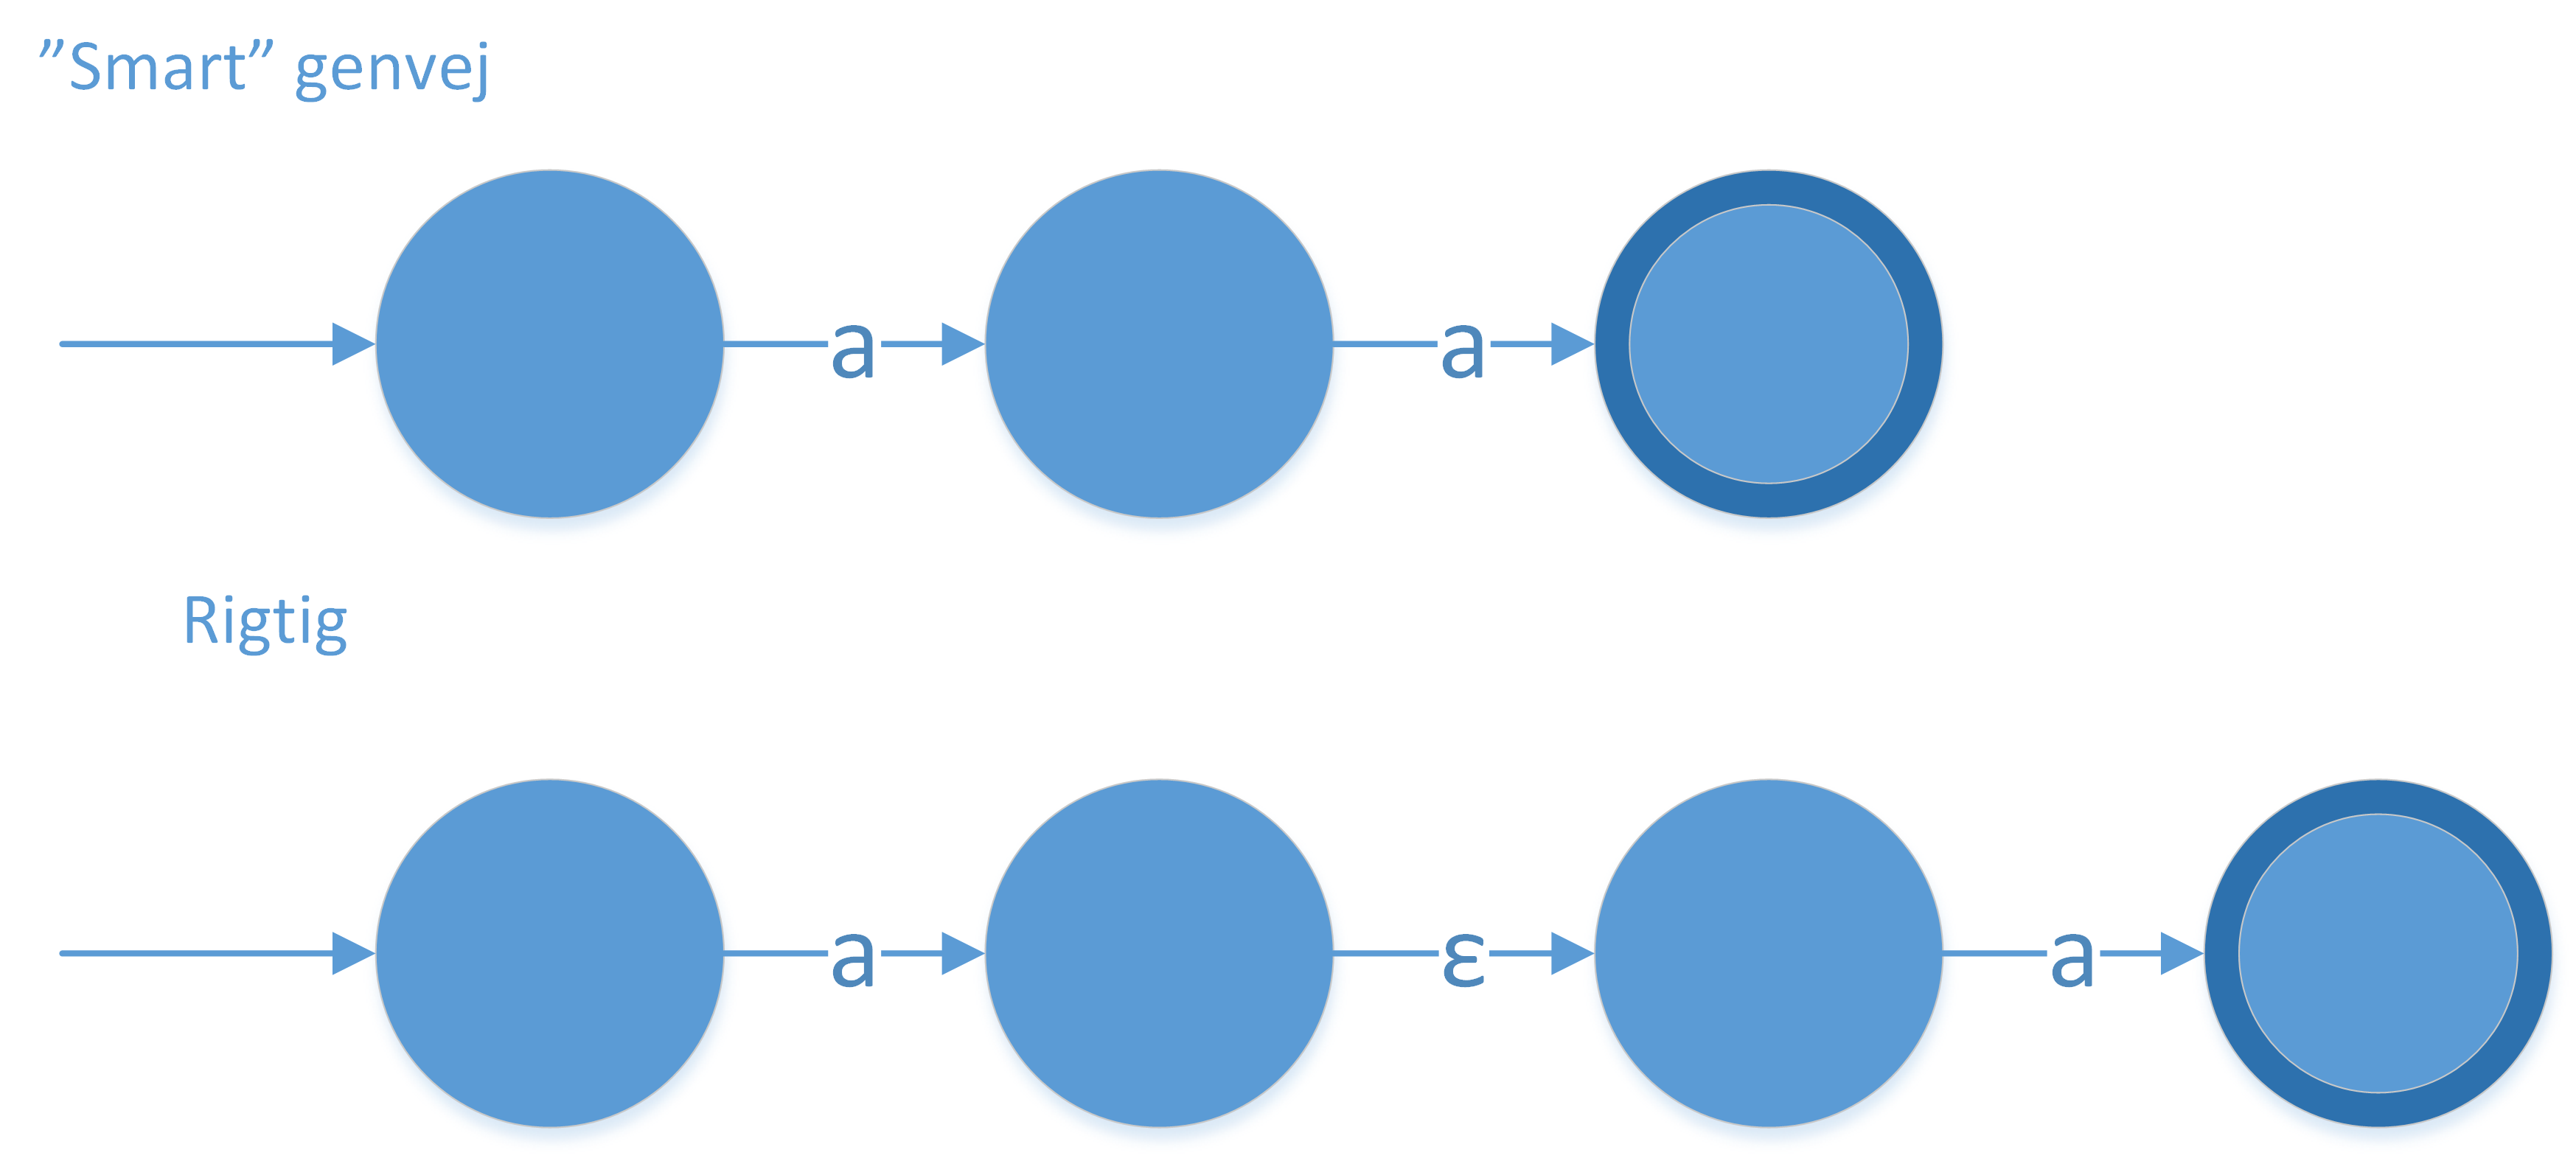
\includegraphics[width=\textwidth]{Fig23x.png}
}
\caption{Undgå smarte genveje som denne.}
\label{fig:fig23}
\end{figure}
\end{document}
